% -*- Mode:TeX -*-

%% IMPORTANT: The official thesis specifications are available at:
%%            http://libraries.mit.edu/archives/thesis-specs/
%%
%%            Please verify your thesis' formatting and copyright
%%            assignment before submission.  If you notice any
%%            discrepancies between these templates and the 
%%            MIT Libraries' specs, please let us know
%%            by e-mailing thesis@mit.edu

%% The documentclass options along with the pagestyle can be used to generate
%% a technical report, a draft copy, or a regular thesis.  You may need to
%% re-specify the pagestyle after you \include  cover.tex.  For more
%% information, see the first few lines of mitthesis.cls. 

%\documentclass[12pt,vi,twoside]{mitthesis}
%%
%%  If you want your thesis copyright to you instead of MIT, use the
%%  ``vi'' option, as above.
%%
%\documentclass[12pt,twoside,leftblank]{mitthesis}
%%
%% If you want blank pages before new chapters to be labelled ``This
%% Page Intentionally Left Blank'', use the ``leftblank'' option, as
%% above. 

\documentclass[12pt,twoside]{mitthesis}
\usepackage{lgrind}
\usepackage{longtable,booktabs,tabularx}
\usepackage{float}
\restylefloat{table}
\pagestyle{plain}
\usepackage{graphicx}
\usepackage{amsmath}
\usepackage{multicol}
\usepackage{multirow}
\usepackage{subfigure}% subcaptions for subfigures
\usepackage{subfigmat}% matrices of similar subfigures, aka small mulitples
\usepackage{fancyvrb}%  extended verbatim environments
\usepackage{bm}
\graphicspath{{./../figs/}}
\usepackage{hyperref}
\usepackage{siunitx}
\usepackage[labelfont=bf,textfont=bf]{caption}
%% This bit allows you to either specify only the files which you wish to
%% process, or `all' to process all files which you \include.
%% Krishna Sethuraman (1990).
%
%\typein [\files]{Enter file names to process, (chap1,chap2 ...), or `all' to process all files:}
%\def\all{all}
%\ifx\files\all \typeout{Including all files.} \else \typeout{Including only \files.} \includeonly{\files} \fi

\begin{document}

% -*-latex-*-
% 
% For questions, comments, concerns or complaints:
% thesis@mit.edu
% 
%
% $Log: cover.tex,v $
% Revision 1.8  2008/05/13 15:02:15  jdreed
% Degree month is June, not May.  Added note about prevdegrees.
% Arthur Smith's title updated
%
% Revision 1.7  2001/02/08 18:53:16  boojum
% changed some \newpages to \cleardoublepages
%
% Revision 1.6  1999/10/21 14:49:31  boojum
% changed comment referring to documentstyle
%
% Revision 1.5  1999/10/21 14:39:04  boojum
% *** empty log message ***
%
% Revision 1.4  1997/04/18  17:54:10  othomas
% added page numbers on abstract and cover, and made 1 abstract
% page the default rather than 2.  (anne hunter tells me this
% is the new institute standard.)
%
% Revision 1.4  1997/04/18  17:54:10  othomas
% added page numbers on abstract and cover, and made 1 abstract
% page the default rather than 2.  (anne hunter tells me this
% is the new institute standard.)
%
% Revision 1.3  93/05/17  17:06:29  starflt
% Added acknowledgements section (suggested by tompalka)
% 
% Revision 1.2  92/04/22  13:13:13  epeisach
% Fixes for 1991 course 6 requirements
% Phrase "and to grant others the right to do so" has been added to 
% permission clause
% Second copy of abstract is not counted as separate pages so numbering works
% out
% 
% Revision 1.1  92/04/22  13:08:20  epeisach

% NOTE:
% These templates make an effort to conform to the MIT Thesis specifications,
% however the specifications can change.  We recommend that you verify the
% layout of your title page with your thesis advisor and/or the MIT 
% Libraries before printing your final copy.
\title{Solar-Electric and Gas Powered, Long-Endurance UAV Sizing via Geometric Programming}

\author{Michael Burton}
% If you wish to list your previous degrees on the cover page, use the 
% previous degrees command:
%       \prevdegrees{A.A., Harvard University (1985)}
% You can use the \\ command to list multiple previous degrees
%       \prevdegrees{B.S., University of California (1978) \\
%                    S.M., Massachusetts Institute of Technology (1981)}
\prevdegrees{B.S., Massachusetts Institute of Technology, 2016}
\department{Department of Aeronautics and Astronautics}

% If the thesis is for two degrees simultaneously, list them both
% separated by \and like this:
% \degree{Doctor of Philosophy \and Master of Science}
\degree{Master of Science in Aeronautics and Astronautics}

% As of the 2007-08 academic year, valid degree months are September, 
% February, or June.  The default is June.
\degreemonth{June}
\degreeyear{2017}
\thesisdate{May 25, 2017}

%% By default, the thesis will be copyrighted to MIT.  If you need to copyright
%% the thesis to yourself, just specify the `vi' documentclass option.  If for
%% some reason you want to exactly specify the copyright notice text, you can
%% use the \copyrightnoticetext command.  
%\copyrightnoticetext{\copyright IBM, 1990.  Do not open till Xmas.}

% If there is more than one supervisor, use the \supervisor command
% once for each.
\supervisor{Warren Hoburg}{Assistant Professor of Aeronautics and Astronautics}

% This is the department committee chairman, not the thesis committee
% chairman.  You should replace this with your Department's Committee
% Chairman.
\chairman{Youssef M. Marzouk}{Associate Professor of Aeronautics and Astonautics\\Chairman, Graduate Program Committee}

% Make the titlepage based on the above information.  If you need
% something special and can't use the standard form, you can specify
% the exact text of the titlepage yourself.  Put it in a titlepage
% environment and leave blank lines where you want vertical space.
% The spaces will be adjusted to fill the entire page.  The dotted
% lines for the signatures are made with the \signature command.
\maketitle

% The abstractpage environment sets up everything on the page except
% the text itself.  The title and other header material are put at the
% top of the page, and the supervisors are listed at the bottom.  A
% new page is begun both before and after.  Of course, an abstract may
% be more than one page itself.  If you need more control over the
% format of the page, you can use the abstract environment, which puts
% the word "Abstract" at the beginning and single spaces its text.

%% You can either \input (*not* \include) your abstract file, or you can put
%% the text of the abstract directly between the \begin{abstractpage} and
%% \end{abstractpage} commands.

% First copy: start a new page, and save the page number.
\cleardoublepage
% Uncomment the next line if you do NOT want a page number on your
% abstract and acknowledgments pages.
% \pagestyle{empty}
\setcounter{savepage}{\thepage}
\begin{abstractpage}
% $Log: abstract.tex,v $
% Revision 1.1  93/05/14  14:56:25  starflt
% Initial revision
% 
% Revision 1.1  90/05/04  10:41:01  lwvanels
% Initial revision
% 
%
%% The text of your abstract and nothing else (other than comments) goes here.
%% It will be single-spaced and the rest of the text that is supposed to go on
%% the abstract page will be generated by the abstractpage environment.  This
%% file should be \input (not \include 'd) from cover.tex.
    Fueled by telecommunication needs and opportunities, there has been a recent push to develop aircraft that can provide long-endurance (days to weeks) persistent aerial coverage.
    These aircraft present a complicated systems engineering problem because of the multifaceted interaction between aerodynamics, structures, environmental effects, and engine, battery, and other component performance.
    Using geometric programming, models capturing the interaction between disciplines are used to analyze the feasible limits of solar-electric and gas powered, long-endurance aircraft in seconds to a level of detail and speed not previously achieved in initial aircraft sizing and design. 
    The results show that long-endurance, gas powered aircraft are generally more robust to higher wind speeds than solar-powered aircraft, but are limited in their endurance by the amount of fuel that they can carry. 
    While solar-electric powered aircraft can theoretically fly for months, they are operationally limited by reduced solar flux during the winter and wind speeds at higher latitudes.
    A detailed trade study between gas-powered and solar-powered aircraft is performed to discover which architecture is best suited to meet a given set of requirements, and what is the optimum size and endurance of that platform.

\end{abstractpage}

% Additional copy: start a new page, and reset the page number.  This way,
% the second copy of the abstract is not counted as separate pages.
% Uncomment the next 6 lines if you need two copies of the abstract
% page.
% \setcounter{page}{\thesavepage}
% \begin{abstractpage}
% % $Log: abstract.tex,v $
% Revision 1.1  93/05/14  14:56:25  starflt
% Initial revision
% 
% Revision 1.1  90/05/04  10:41:01  lwvanels
% Initial revision
% 
%
%% The text of your abstract and nothing else (other than comments) goes here.
%% It will be single-spaced and the rest of the text that is supposed to go on
%% the abstract page will be generated by the abstractpage environment.  This
%% file should be \input (not \include 'd) from cover.tex.
    Fueled by telecommunication needs and opportunities, there has been a recent push to develop aircraft that can provide long-endurance (days to weeks) persistent aerial coverage.
    These aircraft present a complicated systems engineering problem because of the multifaceted interaction between aerodynamics, structures, environmental effects, and engine, battery, and other component performance.
    Using geometric programming, models capturing the interaction between disciplines are used to analyze the feasible limits of solar-electric and gas powered, long-endurance aircraft in seconds to a level of detail and speed not previously achieved in initial aircraft sizing and design. 
    The results show that long-endurance, gas powered aircraft are generally more robust to higher wind speeds than solar-powered aircraft, but are limited in their endurance by the amount of fuel that they can carry. 
    While solar-electric powered aircraft can theoretically fly for months, they are operationally limited by reduced solar flux during the winter and wind speeds at higher latitudes.
    A detailed trade study between gas-powered and solar-powered aircraft is performed to discover which architecture is best suited to meet a given set of requirements, and what is the optimum size and endurance of that platform.

% \end{abstractpage}

\cleardoublepage

\section*{Acknowledgments}

\begin{singlespace}
The success I achieved in completing this thesis a year earlier than expected was only possible because of the incredible support from family, friends, mentors, and MIT faculty.

I first need to thank my family, beginning with my beautiful wife, Jasmine.  
Her support and encouragement have been unwavering.  
When I was up late struggling with a problem, she always believed I would figure it out.  
She has been enthusiastic and supportive of my successes and given sound advice and encouragement when facing difficult problems or situations. 
I could not have done this without her. 

My parents and siblings were also constant sources of support and encouragement. 
My parents are the wisest people I know and I am immensely grateful for their advice.  
They have pushed me to be the best me and I would not have ever made it to MIT without them. 

I want to thank my outstanding advisor, Warren Hoburg (Woody), for his guidance, friendship, and belief in my abilities.  
Woody is a demanding advisor who pushed me to learn, grow, and develop at a pace and intensity that I did not believe possible. 
While rigorous in his pursuit of high quality work, Woody also gave me the flexibility to explore my own interests and taught me to think critically for myself.
He is truly a brilliant professor and a wise mentor and I was fortunate that he selected me to join his lab this year. 

I would not have made it through the rigors and stress of MIT without my best friend and officemate Martin York. 
I could not have shared an office with a more brilliant, passionate and fun person. 
Our common interests, beliefs, and convictions gave me freedom to express my views, opinions, challenges and successes without fear of judgement or offense. 

I also need to thank the project managers, professors, and sponsors of the Jungle Hawk Owl, John Hansmen, Navid Yazdani, Mark Drela, Warren Hoburg and Tony Tao. 
The original problem developed by this team of professionals, of which architecture would was best for the Jungle Hawk Owl was the basis for my thesis work.
They all acted as mentors to me, teaching me technically, guiding me in the industry and giving me opportunities to present my work. 
It was a privilege to work with and for these people to build the Jungle Hawk Owl.

Finally, I want to thank the many fellow students I worked with over the past year and a half building and designing the Jungle Hawk Owl.  
We went through an extremely intense and rapid design and build cycle. 
The late nights, long, arduous layups, and successful test flights have forged a camaraderie between us that I will not forget. 
\end{singlespace}

%%%%%%%%%%%%%%%%%%%%%%%%%%%%%%%%%%%%%%%%%%%%%%%%%%%%%%%%%%%%%%%%%%%%%%
% -*-latex-*-

% Some departments (e.g. 5) require an additional signature page.  See
% signature.tex for more information and uncomment the following line if
% applicable.
% % -*- Mode:TeX -*-
%
% Some departments (e.g. Chemistry) require an additional cover page
% with signatures of the thesis committee.  Please check with your
% thesis advisor or other appropriate person to determine if such a 
% page is required for your thesis.  
%
% If you choose not to use the "titlepage" environment, a \newpage
% commands, and several \vspace{\fill} commands may be necessary to
% achieve the required spacing.  The \signature command is defined in
% the "mitthesis" class
%
% The following sample appears courtesy of Ben Kaduk <kaduk@mit.edu> and
% was used in his June 2012 doctoral thesis in Chemistry. 

\begin{titlepage}
\begin{large}
This doctoral thesis has been examined by a Committee of the Department
of Chemistry as follows:

\signature{Professor Warren Hoburg}{Thesis Supervisor \\
    Assistant Professor of Aeronautics and Astronautics}

\signature{Youssef M. Marzouk}{Chair \\
    Associate Professor of Aeronautics and Astronautics}

\end{large}
\end{titlepage}


\pagestyle{plain}
  % -*- Mode:TeX -*-
%% This file simply contains the commands that actually generate the table of
%% contents and lists of figures and tables.  You can omit any or all of
%% these files by simply taking out the appropriate command.  For more
%% information on these files, see appendix C.3.3 of the LaTeX manual. 
\tableofcontents
\newpage
\listoffigures
% \newpage
\listoftables



\chapter*{Nomenclature}

\begin{tabbing}
  XXXXXXX \= \kill% this line sets tab stop
$A$ \> wing aspect ratio \\
$\bar{A}$ \> non-dimensional wing cross sectional area \\
$A_{\text{h}}$ \> horizontal tail aspect ratio \\
$b$ \> wing span \\ % [ft] \\
BSFC \> brake specific fuel consumption \\ %[kg/kW/hr] \\
$\text{BSFC}_{100\%}$ \> BSFC at full throttle \\ %[kg/kW/hr] \\
$c$ \> wing chord \\ %[m] \\
$\bar{c}$ \> non-dimensional chord \\
$C_D$ \> aircraft drag coefficient \\
$C_{d_0}$ \> non-wing drag coefficient \\
$c_{d_{\text{h}}}$ \> horizontal tail profile drag coefficient \\
$c_{d_p}$ \> wing profile drag coefficient \\
$c_{d_{\text{v}}}$ \> vertical tail profile drag coefficient \\
$C_f$ \> skin friction coefficient \\
$C_L$ \> lift coefficient \\
$(C_{L_{\text{h}}})_{\text{min}}$ \> most-negative allowable horizontal tail lift coefficient \\
$(C_{L_{\text{h}}})_{\delta}$ \> horizontal tail lift coefficient with elevator\\
$c_{l_{\alpha}}$ \> lift slope coefficient \\
$C_{L_{\text{max}}}$ \> maximum lift coefficient \\
$C_{M_{w}}$ \> wing moment coefficient \\
$d$ \> tail boom diameter \\ %[m] \\
$D_{\text{boom}}$ \> tail boom drag \\% [N] \\
$D_{\text{h}}$ \> horizontal tail drag \\% [N] \\
$D_{\text{v}}$ \> vertical tail drag \\% [N] \\
$\Delta W$ \> wing section weight \\ %[N] \\
$\Delta y$ \> wing section length \\ %[m] \\
DOY \> day of the year \\
$e$ \> span efficiency \\
$E$ \> Young's Modulus \\ %[Pa] \\
$E_{\text{batt}}$ \> energy stored in battery \\ %[J] \\
$E_{\text{sun}}$ \> total solar energy available \\ %[Whr] \\
$(E/S)_{\text{twilight}}$ \> twilight solar energy \\ %[Whr/m$^2$] \\
$(E/S)_{\text{day}}$ \> daily required solar energy \\ % [Whr/m$^2$] \\
$(E/S)_{\text{sun}}$ \> available solar energy \\ % [Whr/m$^2$] \\
$\mathcal{F}_{NE}$ \> tail boom flexibility factor \\
$f_{\text{solar}}$ \> planform area fraction covered in solar cells \\
$f_{\text{structural}}$ \> fractional structural weight\\
$g$ \> gravitational constant \\ % [m/s$^2$] \\
$h$ \> flight altitude \\ % [ft] \\
$h_{\text{batt}}$ \> battery specific energy \\ % [Whr/kg] \\
$h_{\text{cap}}$ \> spar cap separation \\ % [m] \\
$\dot{h}_{\text{min}}$ \> minimum climb rate \\ % [ft] \\
$h_{\text{min}}$ \> minimum flight altitude \\
$I$ \> cap spar moment of inertia \\ % [m$^4$] \\
$I_0$ \> tail boom root moment of inertia \\ % [m$^4$] \\
$k$ \> tail boom taper index \\
$K_q$ \> wing loading constant \\ % [N/m$^2$] \\
% $L$ \> atmospheric lapse rate \\ % [K/m] \\
$L_\text{h}$ \> horizontal tail lift \\ % [N] \\
$l_\text{fuse}$ \> fuselage length \\ % [m] \\
$l_\text{h}$ \> horizontal tail moment arm \\ % [m] \\
$l_\text{v}$ \> vertical tail moment arm \\ % [m] \\
$l_\text{w}$ \> wing lift\\ % [m] \\
$m$ \> tail boom mass \\ % [kg] \\
$m'$ \> local wing mass \\ % [kg/m] \\
$\mathcal{M}$ \> wing bending moment \\ % [Nm] \\
$M_{cg}$ \> moment about center of mass \\
% $m_{\text{fac-wing}}$ \> margin factor\\
$m_{\text{fac}}$ \> weight margin factor \\
$\dot{m}_{\text{fuel}}$ \> fuel flow rate \\ % [kg/s] \\
$m_{\text{h}}$ \> horizontal tail span effectiveness \\
$m_{\text{motor}}$ \> electric motor mass \\
$m_w$ \> wing span effectiveness \\
$M_{\text{w}}$ \> moment about wing \\
$n$ \> number of wing segments \\
$N$ \> number of flight segments \\
$N_{\text{max}}$ \> safety load factor\\
% $p$ \> air pressure \\ % [Pa]\\
% $p_{11}$ \> air pressure at 11,000 meters \\ % [Pa]\\
$p_{\text{wind}}$ \> percentile wind speed \\
$P_{0}$ \> magnitude of available solar power \\ % [W/m$^2$] \\
$P_{\text{avionics}}$ \> avionics power \\ % [hp] \\
$P_{\text{oper}}$ \> aircraft operating power \\ % [hp] \\
$(P/S)_{\text{min}}$ \> minimum operational solar power \\ % [Whr/m$^2$] \\
$P_{\text{shaft}}$ \> engine/motor shaft power \\ % [hp] \\
$P_{\text{sun}}$ \> useable solar power per unit area \\ % [W/m$^2$] \\
$P_{\text{sun surface}}$ \> power emitted at the sun's surface \\ % [W/m$^2$] \\
$r_0$ \> average distance from earth to sun \\
$R$ \> aircraft range \\ % [nmi] \\
$R_{\text{earth orbit}}$ \> distance from earth to sun \\
$R_{\text{fuse}}$ \> fuselage radius \\ % [m] \\
$R_{\text{spec}}$ \> specific gas constant \\ % [J/k/K] \\
$R_{\text{sun}}$ \> radius of the sun \\
$q$ \> distributed wing loading \\ % [N/m] \\
$\bar{q}$ \> normalized distributed wing loading \\
$Re$ \> aircraft Reynolds number \\
$Re_{\text{boom}}$ \> tail boom Reynolds number \\
$Re_{\text{h}}$ \> horizontal tail Reynolds number \\
$Re_{\text{v}}$ \> vertical tail Reynolds number \\
$S$ \> wing planform area \\ % [m$^2$]\\
$\mathcal{S}$ \> shear force \\ % [N] \\
$S_{\text{fuse}}$ \> fuselage wetted surface area \\ % [m$^2$]\\
$S_{\text{h}}$ \> horizontal tail planform area \\ % [m$^2$]\\
$S_{\text{solar}}$ \> solar cell area \\ % [m$^2$]\\
$S_{\text{v}}$ \> vertical tail planform area \\ % [m$^2$]\\
$\text{SM}_{\text{min}}$ \> minimum allowable static margin \\
$t$ \> flight time \\ % [days] \\
$t_0$ \> tail boom root wall thickness \\ % [m] \\
$t_{\text{cap}}$ \> spar cap thickness \\ % [m] \\
$t_{\text{day}}$ \> hours of daylight \\ % [hr] \\
$t_{\text{night}}$ \> hours of darkness \\ % [hr] \\
$t_{\text{sun rise}}$ \> time of sun rise \\ % [hr] \\
$t_{\text{sun set}}$ \> time of sun set \\ % [hr] \\
$T$ \> aircraft thrust \\ % [N] \\
% $T_{11}$ \> air temperature at 11,000 meters \\ % [K] \\
% $T_{\text{atm}}$ \> air temperature at flight altitude \\ % [K] \\
% $T_{\text{sl}}$ \> air temperature at sea level \\ % [K] \\
$V$ \> true airspeed \\ % [m/s] \\
$\mathcal{V}_{\text{fuse}}$ \>  fuselage volume \\ % [m$^3$] \\
$V_{\text{gust}}$ \>  gust velocity \\ % [m/s] \\
$V_{\text{h}}$ \> horizontal tail lift coefficient \\
$V_{\text{ref}}$ \>  reference wind airspeed \\ % [m/s] \\
$V_{\text{wind}}$ \>  wind speed \\ % [m/s] \\
$V_{\text{v}}$ \> vertical tail lift coefficient \\
$w$ \> wing deflection \\ % [m] \\
$W$ \> aircraft weight \\ % [N] \\
$W_{\text{ave}}$ \> average weight over a flight segment \\ % [N] \\
$W_{\text{batt}}$ \> battery weight \\ % [N] \\
$w_{\text{cap}}$ \> spar cap width \\ % [m] \\
$W_{\text{cent}}$ \> center of aircraft weight \\ % [N] \\
$W_{\text{emp}}$ \> empennage weight \\ % [N] \\
$W_{\text{engine}}$ \> engine weight \\ % [N] \\
$W_{\text{fadd}}$ \> additional wing structural weight\\ % [N] \\
$W_{\text{final}}$ \> end of flight segment aircraft weight \\ % [N] \\
$W_{\text{fuel}}$ \> fuel weight \\ % [N] \\
$W_{\text{fuselage}}$ \> fuselage weight \\ % [N] \\
$W_{\text{h}}$ \> horizontal tail weight \\ % [N] \\
$W_{\text{initial}}$ \> start of flight segment aircraft weight \\ % [N] \\
$w_{\text{max}}$ \> maximum deflection limit \\ % [m] \\
$W_{\text{motor}}$\> motor weight \\ % [N] \\
$W_{\text{MTO}}$\> max take-off weight \\ % [N] \\
$W_{\text{payload}}$ \> payload weight \\ % [N] \\
$W_{\text{skin}}$ \> wing skin weight \\ % [N] \\
$W_{\text{solar}}$ \> solar cell weight \\ % [N] \\
$W_{\text{spar}}$ \> wing spar weight \\ % [N] \\
$W_{\text{structural}}$ \> structural weight \\ % [N] \\
$W_{\text{v}}$ \> vertical tail weight \\ % [N] \\
$W_{\text{wing}}$ \> wing weight \\ % [N] \\
$x_{ac}$ \> aerodynamic center \\
$(x_{cg})_{\text{aft}}$ \> aft most c.g. position \\
$(x_{cg})_{\text{fwd}}$ \> forward most c.g. position \\
$y$ \> distance from wing root along span \\ % [m] \\
$z_{\text{bre}}$ \> Breguet Range helper variable \\
$\alpha$ \> angle of attack \\
$\alpha_{\text{gust}}$ \> local angle of attack from gust velocities \\ % [rad] \\
$\Delta$ \> solar declination angle \\
$\Delta_{cg}$ \> c.g. travel range \\
$\delta_e$ \> elevator input \\
$\epsilon$ \> downwash angle \\
$\eta_{\text{charge}}$ \> battery charging efficiency \\
$\eta_{\text{discharge}}$ \> battery discharging efficiency \\
$\eta_{\text{motor}}$ \> electric motor efficiency \\
$\eta_{\text{prop}}$ \> propulsive efficiency \\
$\eta_{\text{solar}}$ \> solar cell efficiency \\
$\lambda$ \> wing taper ratio \\
% $\mu$ \> air viscosity \\ % [kg/m/s] \\
% $\mu_0$ \> reference air viscosity \\ % [kg/m/s] \\
$\phi$ \> latitude \\
$\rho$ \> air density \\ % [kg/m$^3$] \\
$\rho_{A_{\text{cfrp}}}$ \> area density of carbon fiber \\ % [kg/cm$^2$] \\
$\rho_{\text{cfrp}}$ \> density of carbon fiber \\ % [kg/cm$^3$] \\
$\rho_{\text{foam}}$ \> density of foam \\ % [lbf/ft$^3$] \\
$\rho_{\text{solar}}$ \> solar cell density \\ % [kg/m$^2$] \\
$\sigma_{\text{cfrp}}$ \> maximum carbon fiber stress \\ % [Pa] \\
$\tau_{\text{h}}$ \> horizontal tail thickness to chord ratio \\
$\tau_t$ \> wing thickness to chord ratio \\
$\tau_{\text{v}}$ \> vertical tail thickness to chord ratio \\
$\tau_w$ \> cap spar width to chord ratio \\
$\theta$ \> angle normal to surface \\
$\theta_{\text{boom}}$ \> tail boom deflection angle \\
$\Theta$ \> wing bending deflection angle 
 \end{tabbing}


\chapter{Introduction}
Long-endurance station-keeping aircraft are potential solutions to providing internet, communication, and persistent aerial coverage. 
Recently, tech companies such as Google\cite{googletitan} and Facebook\cite{aquila} have explored the possibility of using solar-electric powered aircraft to provide internet to parts of the world where 4G or 3G network is not available. 
Engineering firms like Aurora Flight Sciences\cite{orion} and Vanilla Aircraft\cite{vanilla} have developed gas powered long-endurance platforms as a means of providing continual surveillance for days at a time.  
Sizing of such long-endurance aircraft is complicated because of the multifaceted interaction between aerodynamics, structural weight, solar energy, wind speed, and other disciplines and environmental models.
The complexity of sizing these kinds of aircraft makes the trade offs between gas powered and solar-powered architectures potentially non-intuitive. 

This paper presents a physics-based optimization model that uses geometric programming as a systematic and rapid approach to evaluate trade offs between the two architectures for a given mission.  Geometric programming, a form of convex optimization, is chosen as a means of evaluating the design space because of its rapid solve time and guaranteed convergence to a global optimum.\cite{gp}
Models and equations representing the interaction of the various disciplines are expressed in a geometric programming form and are then combined to form an optimization model. 
The optimization can be solved in a fraction of a second and is used quantify to the feasible limits of the solar-electric and gas powered, long-endurance aircraft. 

The driving requirement that sizes solar-electric powered aircraft is the ability to operate at multiple locations and during all seasons.  
To fly multiple days, solar-electric powered aircraft must carry enough solar cells and batteries to fly during the day while storing enough energy to fly through the night.\cite{solartech}
If this condition can be achieved during the winter solstice, when the solar flux is at a minimum, then a solar-electric powered aircraft can theoretically fly during any time of the year for long durations.\cite{solartech}
This becomes more difficult to achieve at higher latitudes as solar flux during the winter solstice decreases.  
Additionally, to station keep the aircraft must fly faster than the local wind speeds.  
Wind speeds are a function of latitude, altitude, and season and tend to increase at higher latitudes and during winter months. 
Therefore, a key sizing study of solar-electric powered aircraft is the effect of latitude on aircraft size.  

The key driving requirement for a gas powered aircraft is endurance.  
As gas-powered aircraft are endurance limited by the amount of fuel that they can carry, longer endurance requires more fuel and hence a larger aircraft.  
Because gas-powered aircraft are not affected by the solar flux, their station-keeping ability at different latitudes only depends on the local wind speed. 
If a gas-powered aircraft can fly at the latitude with the worst wind speed, in can theoretically fly anywhere else in the world.  

Using this geometric programming methodology, trade offs between different aircraft configurations, power sources, and requirements can be calculated in seconds.  
The results show that gas-powered aircraft can generally be built lighter and can fly faster and can therefore fly at higher latitudes and in higher percentile wind speeds.  
Solar-powered aircraft have greater endurance but are limited operationally by their ability to reach higher speeds.  
The presented optimization methodology can quantify the difference in weight and endurance between and gas and solar-electric powered aircraft for the same set of requirements. 
Varying mission requirements reveals how the best architecture changes depending on the requirements. 



\chapter{Mission Requirements}

A comparison of the gas and solar-electric powered aircraft is achieved by comparing their respective capabilities at satisfying a common set of requirements shown in Table~\ref{t:mreqs}.  These requirements can and will be changed in the results section to observe which architecture is best suited to meet various sets of requirements. A discussion of each requirement is included in this section.  

\begin{longtable}{lccccccccccccc}
\caption{Mission Requirements}\\
\toprule
\toprule
\label{t:mreqs}
Payload & 10 lbs\\
Station Keeping & 90\% winds \\
Endurance & $>6$ days\\
Season & all seasons\\
Altitude & $>$ 4,600 m\\
Latitude & $\pm30^{\circ}$\\
\bottomrule
\end{longtable}

\section{Station Keeping}

To station keep an aircraft must fly at least as fast as the wind speed,

\begin{equation}
    \label{e:availreq}
    V \geq V_{\text{wind}}.
\end{equation}

Distributions of wind speed data\cite{wind} indicate that it is impractical for long-endurance UAVs to station keep in 100 percentile wind speeds.  
Therefore, the station keeping requirement is parameterized by a percentile wind speed, $p_{\text{wind}}$, above which the aircraft is allowed to drift off station. 
The wind speed at a station is also a function of latitude, altitude, season or day of the year,

\begin{equation}
    \label{e:windspeed}
    V_{\text{wind}} = f(\phi, h, \text{DOY}, p_{\text{wind}}).
    \end{equation}

Wind speed data was collected from the ERA Interim atmospheric datasets for the years 2005-2015.\cite{wind} 
It is assumed that the wind speed distribution is independent of longitude. 

To meet the season requirement, the solar-electric aircraft must be able to fly a full day/night cycle on the winter solstice.  
If it can do so, it automatically exceeds the endurance requirement. 
To achieve this design constraint the aircraft must be able to fly with limited solar energy, discussed in Section V.B, and with higher than average wind speeds as shown in Figure~\ref{f:windvsmonth}.  

\begin{figure}[h!]
 \begin{subfigmatrix}{2}% number of columns
     \subfigure[+30$^{\circ}$ latitude \label{f:windvsmonthN30}]{\includegraphics[natwidth=560,natheight=420]{windvsmonthN30.pdf}}
     \subfigure[-30$^{\circ}$ latitude \label{f:windvsmonthS30}]{\includegraphics[natwidth=560,natheight=420]{windvsmonthS30.pdf}}
 \end{subfigmatrix}
 \caption{Winds peak at the winter solstice in Northern and Southern Hemispheres.\cite{wind}}
 \label{f:windvsmonth}
\end{figure}

For long-endurance gas powered aircraft, the endurance requirement is the amount of time the aircraft needs to remain in the air without refueling.  
This is expected to be mostly independent of season, except insofar as the wind speeds depends on season. 

Because wind speeds are greatest during the winter solstice for both the Northern and Southern Hemispheres, only wind speeds from December and June, respectively, will be used for the both the gas and solar-electric powered aircraft sizing and performance analysis. 

\section{Altitude}

One altitude requirement is a minimum height required to meet a certain coverage footprint,

\begin{equation}
 h \geq h_{\text{min}}.
\end{equation}

Long-endurance aircraft tend to fly at low speeds, which based on Figure~\ref{f:altvswindhmin} means there are two possible operating altitude regiems: at or around the minimum height requirement of 4,600 m, or at high altitudes between 16,700-20,000 m. 
Gas powered aircraft generally fly in the lower altitude regime of 4,600 m because naturally aspirated engines lose power with increased altitude and are unable to reach altitudes higher than about 13,500 m.  
Solar-electric powered aircraft, which do not have naturally aspirated engines, will fly around 18,000 m to avoid cloud coverage.

\begin{figure}[h!]
	\begin{center}
	\includegraphics[width=0.6\textwidth,natwidth=538,natheight=405]{altvswindhmin.pdf}
    \caption{Aircraft must fly above $h_{\text{min}}$ to meet altitude requirement. Bands represent 80th, 90th and 95th percentiles.\cite{wind}}
	\label{f:altvswindhmin}
	\end{center}
\end{figure}


\section{Latitude}

It is assumed that long-endurance aircraft will have a requirement to be capable of operating anywhere within a band of latitudes.  
For example, an aircraft designed or optimized for the 35th latitude would be able to operate at any latitude between $\pm35$ degrees. 
Latitude affects both the solar-electric and the gas powered aircraft because wind speed varies with latitude. 
Figure~\ref{f:latvswind} shows how the wind speed varies with latitude in the Northern Hemisphere in December. 

\begin{figure}[h!]
	\begin{center}
	\includegraphics[width=0.6\textwidth,natwidth=576,natheight=432]{latvswindN.pdf}
    \caption{Wind speeds by latitude.  Bands represent 80th, 90th and 95th percentile winds.\cite{wind}}
	\label{f:latvswind}
	\end{center}
\end{figure}

Latitude additionally affects the solar-electric powered aircraft because at higher latitudes there is less daylight and therefore less solar energy during the winter months. This is further discussed in Section~\ref{sec:solarenergy}.

\section{Percentile Wind Speed}

For the purposes of this design study, a percentile wind speed corresponds to that percentile of wind speed data across all longitudes in December months spanning the years 2005-2015.  
To understand what a given percentile wind speed implies operationally an autocorrelation analysis was done for multiple cites at varying latitudes at 60,000 during December. 
Figures~\ref{f:bostonwinds} and~\ref{f:romewinds} show the autocorrelation analysis, or the similarity of the next data point to the previous data points, for wind speeds at 60,000 ft over Boston and Rome during December of 2015. 

\begin{figure}[h!]
 \begin{subfigmatrix}{2}% number of columns
     \subfigure[Autocorrelation of Boston wind speeds\label{f:bostonwindatuo}]{\includegraphics[natwidth=560,natheight=420]{Boston_dec_2015auto.pdf}}
     \subfigure[Boston wind speed data\label{f:bostonwind}]{\includegraphics[natwidth=560,natheight=420]{Boston_dec_2015.pdf}}
 \end{subfigmatrix}
 \caption{Wind speed analysis at 60,000 ft over Boston, Massachusetts during December, 2015.}
 \label{f:bostonwinds}
\end{figure}

\begin{figure}[h!]
 \begin{subfigmatrix}{2}% number of columns
     \subfigure[Autocorrelation of Rome wind speeds\label{f:romewindatuo}]{\includegraphics[natwidth=560,natheight=420]{Rome_dec_2015auto.pdf}}
     \subfigure[Rome wind speed data\label{f:romewind}]{\includegraphics[natwidth=560,natheight=420]{Rome_dec_2015.pdf}}
 \end{subfigmatrix}
 \caption{Wind speed analysis at 60,000 ft over Rome, Italy during December, 2015.}
 \label{f:romewinds}
\end{figure}

This analysis shows high wind speeds can last for days at a time.  
An aircraft designed for 90th percentile winds will likely be able to remain on station for 90\% of the time.  
However, during times that wind speeds exceed the 90th percentile they could last for days at a time, possibly requiring the aircraft to drift off station, relocate or land. 

%% This is an example first chapter.  You should put chapter/appendix that you
%% write into a separate file, and add a line \include{yourfilename} to
%% main.tex, where `yourfilename.tex' is the name of the chapter/appendix file.
%% You can process specific files by typing their names in at the 
%% \files=
%% prompt when you run the file main.tex through LaTeX.
\chapter{Geometric Programming}

Sizing long-endurance aircraft for the stated requirements was accomplished using geometric programming. 

\section{Properties of Geometric Programs}

Geometric programs (GPs) are a mathematical optimization problem characterized by the convexity of the objective and constraint functions.\cite{gp} GPs have the form

\begin{align} 
\label{e:gpform}
\text{minimize } f_0(\bm{x}) & \nonumber \\
\text{subject to  } f_i(\bm{x}) &\leq 1, i=1,\ldots,m \\
g_i (\bm{x}) &= 1, i = 1,\ldots,p 
\end{align}

where the functions $g_i$ must be \emph{monomial} functions and the functions $f_i$ must be \emph{posynomial} functions. \emph{Monomials} and \emph{posynomials} have the forms

\begin{align}
 \label{e:mon}
g(\bm{x}) &= c x_1^{a_1} x_2^{a_2} \dotsm x_n^{a_n} , \\
\label{e:pos}
f(\bm{x}) &= \displaystyle\sum_{k=1}^K c_k x_1^{a_{1_k}} x_2^{a_{2_k}} \dotsm x_n^{a_{n_k}}.
\end{align}

The properties of a geometric program allow solution algorithms to guarantee convergence to a global optimum, provided that there exists a feasible solution to the set of constraint functions.  
Additionally, geometric programs can be solved rapidly with existing algorithms.  
Using state of the art, standard interior-point algorithms, GPs with 1,000 variables and 10,000 constraints converge to a solution in tens of seconds.\cite{gp}  

\section{Geometric Program Utilization}

To evaluate the gas and solar-electric powered aircraft design space, the requirements, architecture type, physical models, and assumed parameter values are expressed as constraints on the GP.\cite{hoburgthesis} 
Essentially, the gas and solar-electric powered geometric programs are long lists of constraints in a GP-form that can be solved using interior point methods.  
Figure~\ref{f:flowchart} shows how the optimization problem is constructed and solved. 
The following sections explain in detail the configuration, physical modeling, and input value assumptions and their resulting constraint equations that were used in both the gas and solar-electric powered optimization models.

\begin{figure}[h!]
	\begin{center}
	\includegraphics[width=1.0\textwidth,natwidth=568,natheight=154]{flowchart.eps}
    \caption{Process of constructing and solving a GP optimization problem.}
	\label{f:flowchart}
	\end{center}
\end{figure}

A python package for defining and manipulating geometric programs, GPkit\cite{gpkitdocs}, is used to create the models described in this paper.  
A commercial solver, mosek,\cite{mosek} is used to solve the GP. 
Both the gas and solar-electric powered GP optimization models are available for download and use.\cite{gassolartrade} 


\chapter{Configuration Assumptions}

For this study a simple fixed-wing tractor configuration was chosen as the baseline for both architectures. 
Common characteristics between the gas and solar models include a constant tapered wing and a conventional tail with a single tail boom extending from the wing.  
The gas powered aircraft has a fuselage to hold all of the fuel required for the mission.  
The solar-electric powered aircraft holds the batteries in the wings.  
The solar cells for the solar-electric aircraft are placed along the wing and possibly on the horizontal tail.  
A simple diagram of each vehicle is shown in Figure~\ref{f:simpleaircraft} with their corresponding weight breakdowns in Figure~\ref{f:wbreak}.
The configuration is assumed to be static for this study.

\begin{figure}[h!]
	\begin{center}
	\includegraphics[width=1.0\textwidth,natwidth=447,natheight=265]{simpleaircraft.eps}
    \caption{Blue and red are specific to the solar-electric and gas architectures respectively.  Black are shared characteristics.}
	\label{f:simpleaircraft}
	\end{center}
\end{figure}

\begin{figure}[h!]
	\begin{center}
	\includegraphics[width=1.0\textwidth,natwidth=378,natheight=335]{wbreak.eps}
   \caption{Representative weight breakdown of both aircraft optimization models.}
	\label{f:wbreak}
	\end{center}
\end{figure}


\chapter{Aircraft Physical Models}
\label{chap:phy}

To evaluate the size and performance of both gas and solar-electric powered aircraft, underlying physics models are used.  
Environmental, aircraft performance, and structural models are used in the optimization model to capture the effects of the requirements on the size and design of the aircraft.
Equations from these models are expressed in a GP-compatible form to enable their use in the optimization. 
Understanding the models that are used in a GP is important because the solution to a GP is only as accurate as the models that are used to construct the program.  
To obtain higher fidelity results from the optimization, more detailed models can be implemented. 

\section{Shared Physical Models}

The models described in this section were applied to both the gas powered and solar-electric powered aircraft models. 

\subsection{Steady Level Flight}

Both the gas and solar powered aircraft are assumed to be in steady level flight,\cite{hoburgthesis}

\begin{align}
    \label{e:slfthrust}
    T &\geq \frac{1}{2} \rho V^2 C_D S\\
    \label{e:slfweight}
    W &= \frac{1}{2} \rho V^2 C_L S. 
\end{align}

The shaft power produced by the engine or motor can be expressed as  

\begin{equation}
    \label{e:slfpower}
    P_{\text{shaft}} = \frac{TV}{\eta_{\text{prop}}}
    \end{equation}

    where the propulsive efficiency is assumed to be a constant, $\eta_{\text{prop}} = 0.8$. 

\subsection{Aerodynamics}

The aircraft aerodynamics is modeled as a drag build up of the non-wing drag, wing profile drag, and induced drag coefficients, 

\begin{equation}
    \label{e:aerodragb}
    C_D \geq C_{d_0} + c_{d_p} + \frac{C_L^2}{\pi e A}.
    \end{equation}

where the span efficiency factor is assumed to be constant, $e=0.9$. 
The non-wing drag coefficient $C_{d_0}$, is estimated as a drag build up from the fuselage, tail boom, and horizontal and vertical surfaces discussed later.
    
To estimate the wing profile drag, a posynomial fit is made of the drag polar of the selected \emph{JH01} airfoil, Equation~\ref{e:aerodragprof} (See Appendix \ref{app:jho} for a discussion of the airfoil choice). 
Drag polars were produced using XFOIL\cite{xfoil} at various Reynolds and the data was then fit to a posynomial equation. (See Appendix \ref{app:fits})
    The XFOIL drag polar data is compared to the posynomial fit in Figure~\ref{f:JH01polar}.

    \begin{align}
        \label{e:aerodragprof}
        c_{d_p}^{3.09} &\geq \num{1.02d-7}C_L^{18.86}Re^{-0.18} + 0.0017C_L^{2.93}Re^{-0.66}  \nonumber \\
                       &+ \num{2.28d-6}C_L^{-1.65}Re^{-3.43}+ \num{1.75e8}C_L^{-0.18}Re^{-2.71} \\
        Re &= \frac{\rho V S/b}{\mu}
    \end{align}

\begin{figure}[h!]
	\begin{center}
	\includegraphics[width=0.6\textwidth,natwidth=536,natheight=405]{jho1polarfit1.eps}
    \caption{Posynomial fit (solid lines) to XFOIL data (circles).  (Log-space RMS error~=~0.00489.)}
	\label{f:JH01polar}
	\end{center}
\end{figure}


\subsection{Wing Spar Model}

A wing spar is one of the primary structural elements of both aircraft. 
A conservative approach to calculating the size of the spar is to assume that the spar carries all of the bending loads caused by the lifting loads and weight of the aircraft.  
It is assumed that there are two out of plane bending cases to which both the gas powered and the solar-electric powered aircraft are subject: standard wing bending and gust loads. 

%\begin{itemize}

\subsubsection{Standard Wing Bending Case}
The distributed load along the wing is a combination of the lifting and weight distributions along the wing.
The wing loading distribution $q(y)$, can be approximated as a scaling of the local chord,\cite{bending}

\begin{equation}
    \label{e:wingloading}
    q(y) \approx K_q c(y) 
\end{equation}

where $y$ is the distance from the root wing location. The loading constant $K_q$\cite{bending}, is defined as

\begin{equation}
    \label{e:kq}
    K_q = \frac{N_{\text{max}}W_{\text{cent}}}{S}
\end{equation}

where $W_{\text{cent}}$ is the sum of loads acting at the center of the aircraft and the safety load factor is an input $N_{\text{max}}=5$ ($N_{\text{max}}=1$ corresponds to steady level flight). Using the equation for the local chord of a constant tapered wing\cite{bending} 

\begin{equation}
    \label{e:localchord}
    \bar{c}(y) \equiv \frac{c(y)}{S/b} = \frac{2}{1+\lambda} \left( 1 + (\lambda - 1) \frac{2y}{b} \right)
\end{equation}

where the taper ratio is an input, $\lambda=0.5$.  Thus, the pre-computed distributed load 

\begin{equation}
    \label{e:qbar}
    \bar{q}(y) \equiv \frac{q(y)b}{N_{\text{max}}W_{\text{cent}}} = \frac{2}{1+\lambda} \left( 1 + (\lambda - 1) \frac{2y}{b} \right),
\end{equation}

is inputted into a standard beam model to predict the bending moments and deflections. A diagram depicting this loading case is shown in Figure~\ref{f:gbending}.

\begin{figure}[h!]
	\begin{center}
	\includegraphics[width=0.9\textwidth]{gbending.pdf}
    \caption{Standard g-bending loading case.  Loading scales with local chord.}
	\label{f:gbending}
	\end{center}
\end{figure}

The center weight $W_{\text{cent}}$ for the gas powered aircraft is

\begin{equation}
    W_{\text{cent}} \geq W_{\text{fuel}} + W_{\text{fuselage}} + W_{\text{engine}} + W_{\text{payload}} + W_{\text{emp}}.
\end{equation}

The center weight for the solar powered aircraft is

\begin{equation}
    W_{\text{cent}} \geq W_{\text{payload}} + W_{\text{motor}} + W_{\text{emp}}.
\end{equation}


\subsubsection{Gust Loading Case}

Because long-endurance aircraft typically have high aspect ratio wings, they are considered flexible aircraft. 
To account for this flexibility and size a structural wing spar that will ensure enough rigidity in the event of a gust load, a distributed gust lifting load is added to the steady level flight loading distribution 

\begin{align}
    q(y) &= \frac{N_{\text{max}}W_{\text{cent}}}{b}\bar{c}(y) + c_{l_{\alpha}} \alpha_{\text{gust}} \frac{1}{2} \rho V^2 \frac{S}{b}\bar{c}(y) \\
    \bar{q}(y) = \frac{q(y)b}{W_{\text{cent}}N_{\text{max}}} &\geq \bar{c}(y) \left[1 + \frac{c_{l_{\alpha}}}{C_L} \alpha_{\text{gust}} (y) \left(1 + \frac{W_{\text{wing}}}{W_{\text{cent}}} \right) \right]
\end{align}

where $\bar{c}(y)$ is pre-computed prior to the optimization solve for a taper ratio $\lambda = 0.5$.
The safety load factor is $N_{\text{max}}=2$ for the gust loading case. 
A diagram depicting this loading case is shown in Figure~\ref{f:gust-loading}

\begin{figure}[h!]
	\begin{center}
	\includegraphics[width=0.9\textwidth]{gustloaddiagram.pdf}
    \caption{Gust loading case assumes a 1-cos distribution along the span.}
	\label{f:gust-loading}
	\end{center}
\end{figure}

 The weight of the wing for the gas powered aircraft is assumed to be the weight of the spar cap plus the weight of the skin 

\begin{equation}
    W_{\text{wing}} \geq W_{\text{spar}} + W_{\text{skin}}.
\end{equation}

For the solar-electric powered aircraft the batteries and solar cells are also included in the wing weight

\begin{equation}
    W_{\text{wing}} \geq W_{\text{spar}} + W_{\text{skin}} + W_{\text{batt}} + W_{\text{solar}}.
\end{equation}

The gust velocity is assumed to be vertical to the flight path such that the local angle of attack is approximated by 

\begin{equation}
    \label{e:gustalpha}
    \alpha_{\text{gust}}(y)  = \tan^{-1}\left(\frac{V_{\text{gust}}(y)}{V} \right).
\end{equation}

Because the $\arctan$ function is not GP compatible, a monomial approximation was calculated using techniques described by Hoburg et.~al\cite{fitting}.  The fitted equation is compared to the actual equation in Figure~\ref{f:arctan}

\begin{figure}[h!]
	\begin{center}
	\includegraphics[width=0.6\textwidth,natwidth=547,natheight=74]{arctanfit.pdf}
    \caption{Visual comparison of fitted equation to the arctan function.  (Log space RMS error = 0.039 for $V_{\text{gust}}/V \in [0, 0.7]$)}
	\label{f:arctan}
	\end{center}
\end{figure}

The gust velocity has an assumed profile along the wing\cite{acgust},

\begin{equation}
    \label{e:gustwind}
    V_{\text{gust}}(y) = V_{\text{ref}} \left(1-\cos\left(\frac{2y}{b} \frac{\pi}{2} \right) \right)
\end{equation}

where the reference velocity is an assumed conservative value\cite{acgust}, $V_{\text{ref}} = 10$ [m/s]. The gust velocity profile is computed prior to solve to preserve GP-compatibility.

\subsubsection{Discretized Beam Model}

Using a standard Bernoulli-Euler discretized beam model with $n=5$ nodes\cite{bending}, the shear forces, and moments can be expressed using the distributed loads $q(y)$, as an input with zero forces and moments at the wing tip,

\begin{align}
    \label{e:shear}
    \mathcal{S}_i &= \mathcal{S}_{i+1} - \frac{q_{i+1} + q_i}{2}\Delta y \\
    \label{e:moment}
    M_i &= M_{i+1} - \frac{\mathcal{S}_{i+1} + \mathcal{S}_i}{2}\Delta y \\
    \label{e:shearboundary}
    \mathcal{S}_n &= 0 \\
    \label{e:momentboundary}
    M_n &= 0
\end{align}

Similarly, the angle deflection and deflection can be calculated with boundary conditions of zero angle and deflection and the wing root.\cite{bending}

\begin{align}
    \label{e:angle}
    \Theta_{i} &= \Theta_{i+1} + \frac{1}{2} \left(\frac{M_i}{EI_i} + \frac{M_{i-1}}{EI_{i-1}} \right) \Delta y \\
    \label{e:deflection}
    w_{i} &= w_{i+1} + \frac{1}{2} (\Theta_i + \Theta_{i-1}) \Delta y \\
    \label{e:angleboundary}
    \Theta_0 &= 0 \\
    \label{e:defboundary}
    w_0 &= 0 
\end{align}
 
Equations~\eqref{e:shear}-\eqref{e:defboundary} are GP-compatible if expressed as

\begin{align}
    \label{e:sheargp}
    \mathcal{S}_{i+1} &\geq \mathcal{S}_i + \frac{q_{i+1} + q_i}{2} \Delta y \\
    \label{e:momentgp}
    \mathcal{M}_{i+1} &\geq \mathcal{M}_i + \frac{\mathcal{S}_{i+1} + \mathcal{S}_i}{2} \Delta y \\
    \label{e:anglegp}
    \Theta_{i} &\geq \Theta_{i+1} + \frac{1}{2} \left(\frac{\mathcal{M}_i}{EI_i} + \frac{\mathcal{M}_{i-1}}{EI_{i-1}} \right) \Delta y \\
    \label{e:deflection}
    w_{i} &\geq w_{i+1} + \frac{1}{2} (\Theta_i + \Theta_{i-1}) \Delta y .
\end{align}

where the Young's Modulus of carbon fiber is $E = 20$ [MPa].\\

\subsubsection{Cap Spar for Bending Loads} 
A cap spar is considered for the solar-electric and gas powered aircraft.  A cap spar has two carbon fiber caps separated by a foam core as seen in Figure~\ref{f:capspar}. A thin shear web is wrapped around the caps and foam to prevent shearing and buckling.

\begin{figure}[h!]
	\begin{center}
	\includegraphics[width=0.9\textwidth,natwidth=547,natheight=74]{capsparcross.eps}
    \caption{Cross sectional view of a cap spar.}
	\label{f:capspar}
	\end{center}
\end{figure}

The moment of inertia of the cap spar is modeled by only considering the spar caps, not the foam interior.  
This conservative assumption is made because the contribution of the foam core is much less than that of the spar caps.  
The equation for the moment of inertia\cite{bending} of a cap spar is 

\begin{equation}
    \label{e:moispar}
    I = \frac{w_{\text{cap}}t_{\text{cap}}^3}{6} + 2w_{\text{cap}}t_{\text{cap}}\left( \frac{h_{\text{cap}}}{2} + \frac{t_{\text{cap}}}{2} \right)^2.
\end{equation}

This equation is not GP compatible.  However, using a first order conservative approximation, the moment of inertia can be simplified to be written in a GP-compatible form, 

\begin{equation}
    \label{e:moispar}
    I \leq 2w_{\text{cap}}t_{\text{cap}}\left(\frac{h_{\text{cap}}}{2}\right)^2.
\end{equation}

There are also geometric constraints imposed on the width and thickness.  The total spar cap thickness cannot be greater than the thickness of the airfoil cross section, $\tau_t = 0.115$.  The width of the spar cap is assumed no greater than 30\% of chord, $\tau_w = 0.3$.

\begin{align}
    \label{e:thickness}
    c(y)\tau_t &\geq h_{\text{cap}} + 2t_{\text{cap}} \\
    \label{e:width}
    c(y)\tau_w &\geq w_{\text{cap}} 
    \end{align}

To match the discretized beam model, the spar cross section can also be written in a discretized form such that each section has a unique width and thickness. 

\begin{align}
    I_i &\leq 2w_{\text{cap}_i}t_{\text{cap}_i}\left(\frac{h_{\text{cap}_i}}{2}\right)^2 \\
    c(y)\tau_t &\geq h_{\text{cap}_i} + 2t_{\text{cap}_i} \\
    c(y)\tau_w &\geq w_{\text{cap}_i} 
\end{align}

The wing spar at each section root must be strong enough to withstand the bending moment and stiff enough to not exceed some deflection limit.  Both constraints are imposed in the optimization model as

\begin{align}
    \label{e:stresscont}
    \sigma_{\text{cfrp}} &\geq \mathcal{M}_i \frac{h_{\text{cap}_i}+t_{\text{cap}_i}}{I_i}\\
    \label{e:defcont}
    w_n &\leq w_{\text{max}}
\end{align}

\newpage
where the ultimate tensile strength for unidirectional carbon fiber is $\sigma_{\text{cfrp}} = 1700$ [MPa].\cite{cfprop}
The tip deflection is constrained to be less than 20\% of the half span, $\frac{w_{\text{max}}}{b/2} = 0.2$.

Finally, the weight of the spar cap is computed as

\begin{align}
    \label{e:sparmass}
    \Delta W_i &\geq \rho_{\text{cfrp}} w_{\text{cap}_i}t_{\text{cap}_i} \frac{b/2}{n-1}g \\
    \label{e:sparmasssum}
    W_{\text{spar}} &\geq 2 \sum\limits_{1}^{n-1} \Delta W_i
\end{align}

where $\rho_{\text{cfrp}} = 1.6$ [g/cm$^3$].\cite{cfply}

\subsection{Additional Wing Weight}

It is assumed that the wing skin is made of carbon fiber.  The weight of the wing skin is 

\begin{equation}
    \label{e:wingskinweight}
    W_{\text{skin}} \geq 2 \rho_{A_{\text{cfrp}}} S g.
\end{equation}

where $\rho_{A_{\text{cfrp}}} = 0.049$ [g/cm$^2$], or approximately the area density of one ply of carbon fiber.\cite{cfply} The wing skin is assumed not to contribute to the bending stiffness. 

Additional wing weight $W_{\text{fadd}}$, accounts for additional structural weight (ribs, rear spar, actuators, etc.),

\begin{equation}
    W_{\text{fadd}} \geq (W_{\text{spar}} + W_{\text{skin}}) m_{\text{fac}}
\end{equation}

where $m_{\text{fac}} = 1.2$.


\subsection{Empennage}

An empennage model is added to both the solar-electric and gas powered aircraft models.  The empennage model consists of a single tail boom, horizontal tail and vertical tail.  
The empennage adds both weight and drag to each aircraft.  

The tail boom has an optimized diameter $d$, root wall thickness $t_0$, root moment of inertia $I_0$, modulus $E=150$ [GPa]\cite{cfprop}, density $\rho_{\text{cfrp}} = 1.6$ [g/cm$^3$]\cite{cfprop}, and length $l_{\text{h}}$. 
The total mass and root bending inertia are imposed in the optimization model as 

\begin{align}
    m &\geq \pi \rho_{\text{cfrp}} t_0 d l_{\text{h}} \left( 1 - \frac{1}{2} k\right) \\
    I_0 &\leq \pi t_0 d^3/8
\end{align}

where the index $k=0$ corresponds to a uniform wall thickness and stiffness, and $k=1$ corresponds to a linear drop-off to zero.  For both the solar-electric and gas powered aircraft $k=0.8$ is assumed.  
When the tail boom is loaded at the endpoint $x=l_{\text{h}}$, by the horizontal tail lift $L_{\text{h}}$, the end deflection angle follows from standard beam analysis

\begin{align}
    \label{e:boomdefl}
    \theta &\geq \frac{L_{\text{h}} l_{\text{h}}^2}{EI_0} \frac{1+k}{2} \\
    L_{\text{h}} &= \frac{1}{2} C_{L_{\text{h}}} \rho V^2 S_{\text{h}}.
\end{align}

The horizontal tail is sized to satisfy a horizontal tail volume coefficient condition $V_{\text{h}} = 0.45$,\cite{aircraftrules}

\begin{equation}
    V_{\text{h}} = \frac{S_{\text{h}}l_{\text{h}}}{Sc}
\end{equation}

The vertical tail is sized to meet a conservative tail volume coefficient $V_{\text{v}}= 0.04$,\cite{aircraftrules}

\begin{equation}
    \label{e:vtv}
    V_{\text{v}} = \frac{S_{\text{v}}}{S} \frac{l_{\text{v}}}{b}
\end{equation}

where $l_{\text{v}}$ is the vertical tail moment arm, assumed to be equal to the horizontal tail moment arm, $l_{\text{v}} = l_{\text{h}}$.

Both the horizontal and vertical tails are assumed to have a carbon fiber skin and solid foam interior where their respective densities are $\rho_{A_{\text{cfrp}}} = 0.049$ [g/cm$^2$], $\rho_{\text{foam}} = 1.5$ [lbf/ft$^3$]. 
The weight of the tails is

\begin{equation}
    W_{\text{(v,h)}}/m_{\text{fac}} = \rho_{\text{foam}} \frac{S_{\text{(v,h)}}^2}{b_{\text{(v,h)}}} \bar{A} + g\rho_{A_{\text{cfrp}}} S_{\text{(v,h)}} \\
\end{equation}

where $b_{\text{h}}$ and $b_{\text{v}}$ are the spans of the horizontal and vertical tails respectively and $\bar{A}$ is the cross sectional area of the NACA 0008 airfoil. The margin factor $m_{\text{fac}}=1.1$, is included to account for control surfaces, attachment joints, actuators, etc. 

The drag of the empennage was modeled as three separate parts with no interference drag.  The drag of the tail boom is calculated using a turbulent flat plate model,

\begin{align}
    \label{e:boomdrag}
    D_{\text{boom}} &\geq \frac{1}{2} C_f \rho V^2 l_{\text{h}}\pi d \\
    C_f &\geq \frac{0.445}{Re_{\text{boom}}^{0.3}} \\
    Re_{\text{boom}} &= \frac{V\rho l_{\text{h}}}{\mu}
\end{align}

The drag of the horizontal and vertical tails is computed using a multiple monomial equations fitted from XFOIL data for a range of Reynolds numbers and NACA airfoil thicknesses,

\begin{align}
    D_{\text{(v,h)}} &\geq \frac{1}{2} c_{d_{\text{(v,h)}}} \rho V^2 S_{\text{(v,h)}} \\
    \label{e:taildrag}
    c_{d_{\text{(v,h)}}} &\geq 0.34 Re_{\text{(v,h)}}^{-0.18} \tau_{\text{(v,h)}}^{0.77} \\
    c_{d_{\text{(v,h)}}} &\geq 5.45 Re_{\text{(v,h)}}^{-0.48} \tau_{\text{(v,h)}}^{0.25} \\
    c_{d_{\text{(v,h)}}} &\geq 16.3 Re_{\text{(v,h)}}^{-0.54} \tau_{\text{(v,h)}}^{0.47} \\
    c_{d_{\text{(v,h)}}} &\geq 9.51 Re_{\text{(v,h)}}^{-0.48} \tau_{\text{(v,h)}}^{0.47} \\
    \label{e:taildragend}
    c_{d_{\text{(v,h)}}} &\geq 218.7 Re_{\text{(v,h)}}^{-0.60} \tau_{\text{(v,h)}}^{1.31} \\
    Re_{\text{(v,h)}} &= \frac{\rho V S_{\text{(v,h)}}/b_{\text{(v,h)}}}{\mu}
\end{align}

where the selected airfoil is the NACA 0008 for both the horizontal and vertical tails (i.e. $\tau_{\text{(v,h)}} = 0.08$). 
The XFOIL data was generated for a zero angle of attack, based upon steady level flight where neither surface is generating lift.  
A comparison of the XFOIL data and Equations~\eqref{e:taildrag}-\eqref{e:taildragend} is shown in Figure~\ref{f:taildragpolar}.

\begin{figure}[H]
	\begin{center}
	\includegraphics[width=0.6\textwidth,natwidth=538,natheight=405]{taildragpolar.pdf}
    \caption{Posynomial fit (solid lines) to XFOIL data (circles). (Log-space RMS error = 0.040)}
	\label{f:taildragpolar}
	\end{center}
\end{figure}


\section{Solar-Electric Aircraft Physical Models}

\subsection{Wind Speeds}

There exists an optimum flight altitude for solar-electric powered aircraft.  
The local minimum in wind speed around 19,000 m and the variation of air density with altitude suggest that the altitude should be an output of the optimization. 
To accomplish this, constraints relating wind speed to altitude are imposed. 
This approach assumes that the solar-electric powered aircraft will not be confined to fly at a single altitude, but will fly at the altitude where conditions are most favorable.

Because wind speeds do not increase monotonically with latitude, it is possible that the design for a given latitude is constrained by winds at a latitude inside the required latitude band. 
To handle this, a multipoint set of latitude constraints is imposed. 
The wind speed data used to generate these equations includes December wind speeds from the Northern Hemisphere and June wind speeds from the Southern Hemisphere for the years 2005-2015.
In total, 41 wind speed constraints were generated to represent $\pm$20-60 degrees each with a log space RMS error of less than 5\%. (See Appendix \ref{app:fits}) The wind constraint at 30 degrees latitude is shown in Figure~\ref{f:windfitl30}

\begin{figure}[H]
	\begin{center}
	\includegraphics[width=0.6\textwidth,natwidth=511,natheight=405]{windfitl30.pdf}
    \caption{Posynomial approximation to wind speed data\cite{wind} (circles) at 30$^{\circ}$ latitude. (Log-space RMS error = 0.047.)}
	\label{f:windfitl30}
	\end{center}
\end{figure}

For the gas powered aircraft, the altitude is not optimized.  
Gas-powered aircraft, which are naturally aspirated, will be less efficient at higher altitudes.  
Additionally, wind speeds increase monotonically from sea level up to $\sim$9,100 m.  
Therefore, the altitude for gas-powered aircraft is determined as the minimum altitude necessary for the payload to be effective.\cite{orion}
For this sizing study, the altitude requirement for the gas powered aircraft is $h_{\text{min}}=4,500$ m, corresponding to a 100 km diameter footprint with a 5 degree lookup angle. 

\subsection{Solar-Electric Power}
\label{sec:solarenergy}

At a given time of year DOY, and latitude $\phi$, there exists an available solar irradiated energy $(E/S)_{\text{sun}}$ per unit area during one day,

\begin{equation}
    \label{e:solarfunc}
    (E/S)_{\text{sun}} = f(\phi, \text{DOY}).
\end{equation}

To operate continually for multiple days the total available solar energy $(E/S)_{\text{sun}}$, must be greater than the required pre-conversion-efficiency solar energy per unit area to power the aircraft during the day $(E/S)_{\text{day}}$, and the energy required to power the aircraft during the night via batteries $E_{\text{batt}}$,\cite{solartech}

\begin{align}
    \label{e:solarreq}
    (E/S)_{\text{sun}}  &\geq (E/S)_{\text{day}} + \frac{E_{\text{batt}}}{\eta_{\text{charge}}\eta_{\text{solar}} S_{\text{solar}}} \\
    \label{e:solarbatt}
    E_{\text{batt}} \eta_{\text{discharge}} &\geq P_{\text{oper}}t_{\text{night}} + (E/S)_{\text{twilight}} \eta_{\text{solar}} S_{\text{solar}}
\end{align}

where the charge, discharge and solar cell efficiencies are assumed to be $\eta_{\text{charge}} = \eta_{\text{discharge}} = 0.98$ and $\eta_{\text{solar}}= 0.22$. 
An additional energy term $(E/S)_{\text{twilight}}$ is included in Equation~\eqref{e:solarbatt} to account for hours of low solar irradiance, during mornings and evenings, when the aircraft must continue to fly on partial battery power. 
Equations~\eqref{e:solarreq} and~\eqref{e:solarbatt} are graphically represented in Figure~\ref{f:lat30}, which represents the solar energy at 30 degrees latitude. 

\begin{figure}[h!]
	\begin{center}
	\includegraphics[width=0.7\textwidth,natwidth=572,natheight=405]{lat30.pdf}
    \caption{Solar power on Dec 21st at 30$^{\circ}$ North. 24-hour operationality achieved when red area exceeds blue, magenta and green areas. }
	\label{f:lat30}
	\end{center}
\end{figure}

In order for the aircraft to begin charging batteries there must be a minimum solar irradiance power

\begin{align}
    (P/S)_{\text{min}} &= \frac{P_{\text{oper}}}{\eta_{\text{solar}} S_{\text{solar}}} \\
    \eta_{\text{motor}} P_{\text{oper}} &\geq P_{\text{shaft}} + P_{\text{avionics}}.
\end{align}

where $\eta_{\text{motor}} = 0.95$. 
Thus, for a given latitude and day, and therefore total solar energy $(E/S)_{\text{sun}}$, both $(E/S)_{\text{day}}$ and $(E/S)_{\text{twilight}}$ are functions of $(P/S)_{\text{min}}$.  
The total solar energy available $(E/S)_{\text{sun}}$, is computed prior to the optimization solve and is used to generate monomial approximations for $(E/S)_{\text{day}}$ and $(E/S)_{\text{twilight}}$ as functions $(P/S)_{\text{min}}$, one for each degree of latitude between 20 and 60 degrees latitude. 
$(E/S)_{\text{sun}}$, $(E/S)_{\text{day}}$, $(E/S)_{\text{twilight}}$, and $t_{\text{night}}$ are precomputed using the formulas in Appendix \ref{app:solar} to generate the fitted equations. 
Figure~\ref{f:energyapprox} shows sample monomial approximations of the twilight and day energy equations at 30 degrees latitude. 

\begin{figure}[H]
 \begin{subfigmatrix}{2}% number of columns
     \subfigure[Monomial Approxmiation for $(E/S)_{\text{day}}$\label{f:Benergy}]{\includegraphics[natwidth=576,natheight=432]{Benergy.pdf}}
     \subfigure[Monomial Approximation for $(E/S)_{\text{twilight}}$\label{f:Cenergy}]{\includegraphics[natwidth=575,natheight=432]{Cenergy.pdf}}
 \end{subfigmatrix}
 \caption{Monomial approximations for $(E/S)_{\text{day}}$ and $(E/S)_{\text{twilight}}$. (Log-space RMS error = 0.007 and 0.0180)}
 \label{f:energyapprox}
\end{figure}


For the purposes of this design study, it is assumed that the solar cells are placed on the wing and the horizontal tail but not on the vertical tail. 
The fractional solar cell area index $f_{\text{solar}}$ is one when the solar cells completely cover the main wing and greater than one if solar cells are also placed on the horizontal tail,

\begin{equation}
    \label{e:solarssolar}
    S_{\text{solar}} \leq f_{\text{solar}}S.
\end{equation}

\subsection{Motor Weight}

The solar-electric powered aircraft has a motor whose weight is based on the approximation\cite{electricengine}

\begin{equation}
    \label{e:electricengine}
    P_{\text{max}} = B_{\text{PM}} m_{\text{motor}}
\end{equation}

where $m_{\text{motor}}$ is the motor mass, $P_{\text{max}} \geq P_{\text{oper}}$ is the maximum operating power, and the assumed power to mass ratio is $B_{PM} = 4140.8$ [W/kg]. \\

\section{Gas Powered Aircraft Physical Models}

\subsection{Breguet Endurance}

A key sizing equation for a long endurance gas powered aircraft is the Breguet Range equation.  
For GP-compatibility and to optimize endurance, not range, a variation of the Breguet Range equation is used, 

\begin{equation}
    \label{e:breguetendurance}
    t = \frac{W_{\text{ave}}}{P_{\text{shaft}}\text{BSFC}g} \ln{\left( \frac{W_{\text{initial}}}{W_{\text{final}}}\right)}.
\end{equation}

The derivation of this form begins with the differential form of Breguet Range,\cite{br2}

\begin{equation}
    \label{e:breguetdiff}
    -\frac{dW}{dt} = g\dot{m}_{\text{fuel}}.
\end{equation}

Using the definition of $\text{BSFC}$

\begin{equation}
    \label{e:brBSFC}
    \text{BSFC} = \frac{\dot{m}_{\text{fuel}}}{P_{\text{shaft}}},
\end{equation}

Equation~\eqref{e:breguetdiff} can be written as

\begin{equation}
    \label{e:brdiff2}
    -dW = g P_{\text{shaft}} \text{BSFC} dt.
\end{equation}

Dividing by $W$,

\begin{equation}
    \label{e:brdiff2}
    -\frac{dW}{W} = \frac{g P_{\text{shaft}}\text{BSFC} }{W} dt,
\end{equation}

and integrating, the Breguet Range equation can be expressed as

\begin{equation}
    \label{e:be1}
    \ln{\left( \frac{W_{\text{initial}}}{W_{\text{final}}} \right)} = \frac{gP_{\text{shaft}}\text{BSFC}}{W_{\text{ave}}} t,
\end{equation}
 
where the segment weight $W_{\text{ave}}$, is assumed to be the geometric mean, defined as

\begin{equation}
    \label{e:gpmean}
    W_{\text{ave}} = \sqrt{W_{\text{initial}}W_{\text{final}}}.
\end{equation}

This version of the Breguet Range equation comes from assuming that $\text{BSFC}$ and the power to weight ratio, $(P_{\text{shaft}}/W)$, are constant during the considered flight segment. 
One way to obtain a constant power to weight ratio is a constant velocity and constant lift coefficient.\cite{br2}

    To make Equation~\eqref{e:breguetendurance} GP compatible, a Taylor expansion is used,\cite{hoburgthesis}

\begin{align}
    \label{e:brzbre}
    z_{\text{bre}} &\geq \frac{P_{\text{shaft}}t \text{BSFC} g}{W}\\
    \label{e:brtaylor}
    \frac{W_{\text{fuel}}}{W_\text{final}} &\geq z_{\text{bre}} + \frac{z_{\text{bre}}^2}{2} + \frac{z_{\text{bre}}^3}{6} + \frac{z_{\text{bre}}^4}{24} + \dots
\end{align}

    Equations~\eqref{e:brzbre} and~\eqref{e:brtaylor} are monomial and posynomial respectively and therefore GP compatible. For long-endurance aircraft, missions can last days, causing the power to weight ratio $(P_{\text{shaft}}/W)$ to vary significantly during the course of the flight.  
    Equations~\eqref{e:slfweight}~,\eqref{e:brzbre}, and~\eqref{e:brtaylor} can be discretized to account for this,

\begin{align}
    \label{e:slfweightd}
    \sqrt{W_i W_{i+1}} &= \frac{1}{2} \rho_i V_i^2 C_{L_i} S \\
    \label{e:brzbred}
    z_{bre_i} &\geq \frac{P_{\text{shaft}_i}t_i \text{BSFC} g}{\sqrt{W_i W_{i+1}}}\\
    \label{e:brtaylord}
    \frac{W_{\text{fuel}_i}}{W_{i+1}} &\geq z_{bre_i} + \frac{z_{bre_i}^2}{2} + \frac{z_{bre_i}^3}{6} + \frac{z_{bre_i}^3}{24}.
    \end{align}

    For evaluation of long-endurance, gas-powered aircraft a discretization of $N=5$ was used. 

\subsection{Elliptical Fuselage}

For the gas powered aircraft it is assumed that the fuel is carried in an elliptically shaped fuselage.  The fuselage will increase the overall weight and drag of the aircraft.  The solar-electric powered aircraft is assumed to carry the batteries in the wings and will therefore have a small fuselage whose effects will be ignored.  

The driving constraint for the size of the fuselage is to ensure that all of the fuel required for the mission can fit inside the fuselage, 

\begin{equation}
    \label{e:fusevol}
    \mathcal{V}_{\text{fuse}} \geq \frac{W_\text{fuel}}{\rho_\text{fuel}}
\end{equation}

where the fuel is assumed to have a density $\rho_\text{fuel} = 6.01$ [lbf/gallon].  The dimensions of the fuselage are constrained by

\begin{equation}
    \label{e:fusevol2}
    \mathcal{V}_{\text{fuse}} \leq \frac{4}{3}\pi \frac{l_{\text{fuse}}}{2}R_{\text{fuse}}^2
\end{equation}

where $l_{\text{fuse}}$ is the length of the fuselage and $R_{\text{fuse}}$ is the radius. Using the length and radius, the surface area can be calculated using Thomsen's approximation,\cite{ellipsoidSA}

\begin{equation}
    \label{e:fusesa}
    3 \left( \frac{S_{\text{fuse}}}{\pi} \right)^{1.6075} \geq 2(2l_{\text{fuse}}R_{\text{fuse}})^{1.6075} + (4R_{\text{fuse}}^2)^{1.6075}.
\end{equation}

The weight of the fuselage is constrained by

\begin{equation}
    \label{e:fuseweight}
    W_{\text{fuse}} \geq S_{\text{fuse}} \rho_{A_{\text{cfrp}}} g
\end{equation} 

where $\rho_{A_{\text{cfrp}}} = 0.0975$ [g/cm$^2$], or the area density of two plies of carbon fiber.\cite{cfply}  The surface area is also used to calculate the drag assuming a skin friction based drag model,

\begin{align}
    \label{e:fusedrag}
    D_{\text{fuse}} &\geq C_f k_{\text{fuse}} \frac{1}{2} \rho V^2 S_{\text{fuse}} \\
    C_f &\geq \frac{0.455}{Re^{0.3}}
\end{align}

where $k_{\text{fuse}}$ is the form factor approximated by\cite{raymer}

\begin{equation}
    \label{e:fuseform}
    k_{\text{fuse}} \geq 1 + \frac{60}{(l_{\text{fuse}}/2R_{\text{fuse}})^3} + \frac{(l_{\text{fuse}}/2R_{\text{fuse}})}{400}.
\end{equation}

\subsection{Engine Weight}

The engine weight of the gas powered aircraft is governed by a simple power law derived from existing two-stroke and four-stroke engines\cite{gasengine}

\begin{equation}
    \label{e:powerlaw}
    \frac{W_{\text{engine}}}{W_{\text{engine-ref}}} = 1.27847 \left(\frac{P_{\text{SL-max}}}{P_{\text{ref}}} \right)^{0.772392}
\end{equation}

where $W_{\text{engine-ref}} = 10$ [lbs] and $P_{\text{ref}} = 10$ [hp].   
Equation~\eqref{e:powerlaw} is compared to the data in Figure~\ref{f:powervsweightfit}.

\begin{figure}[h!]
	\begin{center}
	\includegraphics[width=0.6\textwidth,natwidth=524,natheight=405]{powervsweightfit.eps}
    \caption{Power law fit to University of North Dakota engine weight data\cite{gasengine}. (Log-space RMS error = 0.34)}
	\label{f:powervsweightfit}
	\end{center}
\end{figure}

\subsection{Engine Performance}

Two characteristics of gas engines affect the performance of long-endurance aircraft.  
The first is brake specific fuel consumption, $\text{BSFC}$; a lower $\text{BSFC}$ will result in increased endurance.  
The second is the lapse rate.  
Assuming a propeller driven aircraft and a naturally aspirated engine, as the aircraft reaches higher altitudes, the engine will have decreased available power. 
To account for these two effects a two-stroke, double cylinder engine, the DF70 from RCV Engines Ltd, England, was selected as a representative engine.  
RCV Engines Ltd provided manufacturing data that was used to generate representative performance curves.\cite{rcvengines}
It is assumed that engines of a similar size will perform similarly to the DF70 engine.  
This engine performance model is only valid for internal combustion engines.

To capture throttling effects as aircraft weight decreases, a GP-compatible curve was generated from the DF70 data to relate $\text{BSFC}$ and shaft power. 
A comparison of the GP approximation, Equation~\eqref{e:rpmtobsfc}, and the DF70 engine data is shown in Figure~\ref{f:powertobsfc}.
Using this approximation the required shaft power determines the $\text{BSFC}$.
A comparison of the DF70 data provided by RCV Engine Ltd in Figure~\ref{f:powertobsfc} to the $\text{BSFC}$ to power curves in Goering\cite{bsfcperf} verify that this performance curve is representative of engines of similar sizes. 

\begin{align}
    \left( \frac{\text{BSFC}}{\text{BSFC}_{100\%}} \right)^{18.5563} &\geq \num{8.66321d-3}\left( \frac{P_{\text{shaft}}}{P_{\text{max}}}\right)^{-7.70161} \nonumber \\
    \label{e:rpmtobsfc}
                &+ 1.38628\left( \frac{P_{\text{shaft}}}{P_{\text{max}}} \right)^{1.12921} 
\end{align}

where $\text{BSFC}_{100\%} = 0.3162$ [kg/kW/hr].\cite{rcvengines}

\begin{figure}[h!]
	\begin{center}
	\includegraphics[width=0.6\textwidth,natwidth=530,natheight=414]{powertobsfcfit.eps}
    \caption{Representative engine performance fit based on RCV Engine Ltd data.  (Log-space RMS error = 0.007) }
	\label{f:powertobsfc}
	\end{center}
\end{figure}

The lapse rate $L_{\text{eng}}(h) \leq 1$, is assumed to affect the maximum power output,

\begin{equation}
    \label{e:lapse}
    L_{\text{eng}}(h) \equiv \frac{P_{\text{max}}}{P_{\text{SL-max}}}.
\end{equation}

The lapse is calculated from the required flight altitude $h=4,500$ [m], prior to the optimization solve using an approximate engine loss rate for normally aspirated engines of 3.5\% hp per 300 m,\cite{enginelapse}

\begin{equation}
    \label{e:lapsefit}
    L_{\text{eng}}(h) = 1 - \frac{0.035}{300 \text{ [m]}} h.
\end{equation}

\subsection{Climb Constraints}

Because the gas engine is naturally aspirated, as the aircraft climbs there will be less available power.  
The climb constraint ultimately sizes the engine because at the top of climb, when the least amount of power is available, the engine must provide the necessary power to meet a minimum climb rate, 

\begin{equation}
    \label{e:climbrate}
    \dot{h}_{\text{min}} \geq 30 \text{ [m/min]}.
\end{equation}

The climb rate affects the required thrust, and therefore the required power during climb, 

\begin{equation}
    \label{e:climb}
    T \geq \frac{1}{2} C_D \rho V^2 S + W \frac{\dot{h}_{\text{min}}}{V}
\end{equation}

where $W$ is the weight of the aircraft during climb.  


\chapter{Results}

The gas and solar-electric powered aircraft optimization models were solved by minimizing the take-off weight for the requirements listed in Table~\ref{t:mreqs} and the assumptions and key design parameters described herein. 
The solar-electric powered optimization model had 375 unknowns and was solved in 0.164 seconds for a max take-off weight of 192 lbs.
The gas powered aircraft optimization model had 552 unknowns and was solved in 0.144 seconds for a max take-off weight of 72.3 lbs.  
Important design parameters are listed in Table~\ref{t:gassolarparams}.
Key design variables for both architectures are listed in Tables~\ref{t:svals} and~\ref{t:gvals} for various mission requirements. 
The rest of this section explores how these result may vary for different requirements, input parameter values, and physics modeling assumptions. 

\footnotesize
\begin{longtable}{llll}
\caption{Fixed Optimization Parameters} \\
\toprule
\toprule
\multicolumn{2}{c}{Gas Powered} & \multicolumn{2}{c}{Solar Powered}\\
\midrule
$\eta_{\text{prop}}$         & 0.8  & $\eta_{\text{prop}}$         & 0.8 \\
$\tau$                       & 0.115 & $\tau$                       & 0.115 \\
$\lambda$                    & 0.5  & $\lambda$                    & 0.5 \\
$\sigma_{\text{CFRP}}$ [MPa] & 1700 & $\sigma_{\text{CFRP}}$ [MPa] & 1700  \\
$N_{\text{max}}$ - g-Loading & 5    & $N_{\text{max}}$ - g-Loading & 5 \\
$N_{\text{max}}$ - gust load & 2    & $N_{\text{max}}$ - gust load & 2 \\
$\text{BSFC}_{100\%}$ [kg/hr/kW] & 0.31 & $\eta_{\text{solar}}$      & 0.22 \\
Lapse Rate [hp/1000 ft]      & 0.035 &  $h_{\text{batt}}$ [Whr/kg]   & 350 \\
$\dot{h}_{\text{min}}$ [ft/min] & 100 & $\eta_{\text{motor}}$           & 0.95 \\ 
$\rho_{\text{fuel}} $ [lbf/gallon] & 6.01 & $\eta_{\text{charge}}$          & 0.98 \\
                             &     & $\eta_{\text{discharge}}$       & 0.98 \\
\bottomrule
\label{t:gassolarparams}
 \end{longtable}

\input{../svals.generated.tex}
\input{../gvals.generated.tex}

\normalsize

\section{Changing Requirements}

Important trade offs between the gas powered and solar-electric powered architectures are highlighted and quantified by changing the latitude and endurance requirements.   

\subsection{Latitude Requirement Analysis}

Both optimization models were solved by minimizing the max take-off weight across different latitude requirements. 
Figure~\ref{f:latvsmtowtrade} shows this result evaluated at the 80th, 90th and 95th percentile wind speeds.  
The gas powered model was solved 63 times in 5.6178 seconds total and the solar-electric powered model was solved 31 times in 2.5529 seconds total to produce Figure~\ref{f:latvsmtowtrade}.

\begin{figure}[h!]
	\begin{center}
	\includegraphics[width=0.7\textwidth,natwidth=528,natheight=405]{mtowvslat.pdf}
    \caption{Gas architecture feasible for all latitudes. Next integer latitude for each solar-electric curve is infeasible.}
    \label{f:latvsmtowtrade}
	\end{center}
\end{figure}

One way to interpret Figure~\ref{f:latvsmtowtrade} is that a solar-powered aircraft weighing 190 lbs is able to operate between $\pm$28 degrees latitude in 90th percentile wind speeds.  
This analysis shows that gas powered architectures are able to operate in more locations than solar-electric powered aircraft.  
On the other hand, solar-electric powered aircraft design becomes infeasible at higher latitudes because even though wind speeds peak around 42 degrees latitude at 18,300 m, the combination of lower solar flux and higher wind speeds makes it difficult to reach latitude bands greater than $\pm$30 degrees. 

\subsection{Endurance Requirement Analysis}
While the solar-electric powered aircraft may be limited operationally by higher latitudes, it is not limited in endurance as is the gas powered aircraft.
Solving the gas powered optimization model for different endurance requirements shows where the gas powered architecture becomes less feasible. 
Figure~\ref{f:mtowvsendurance} shows the endurance versus size analysis for a gas powered aircraft by minimizing max take-off weight for an aircraft capable of flying at any latitude. 
Figure~\ref{f:mtowvsendurance} was generated using 29 separate optimization solutions that took a total of 2.403 seconds to solve.

\begin{figure}[h!]
	\begin{center}
	\includegraphics[width=0.7\textwidth,natwidth=527,natheight=405]{mtowvsendurance.pdf}
    \caption{Endurance and size trade study for gas powered architecture.}
	\label{f:mtowvsendurance}
	\end{center}
\end{figure}

\subsection{Season Requirement Analysis}

The season requirement for the solar-electric powered aircraft if met, allows for year round coverage.  
However, there may be applications that require flying for only 10 months of the year or even half the year.  
Figure~\ref{f:season} shows which latitudes are feasible for different season requirements and what the aircraft weight would be. 
Interestingly, flying for only 10 months of the year does not increase the ability to reach higher latitudes.  
However, there is considerable benefit to only flying for 6 months of the year.  

\begin{figure}[h!]
	\begin{center}
	\includegraphics[width=0.6\textwidth,natwidth=527,natheight=405]{season.pdf}
    \caption{Flexible season requirements allow for smaller aircraft and increased latitude.}
	\label{f:season}
	\end{center}
\end{figure}

\section{Changing Parameter Values}

The previous results are dependent on the assumed input values and parameters.  
Changing parameter values can help show where the designs becomes infeasible. 
As one example, two input values that are especially important to the solar aircraft are the solar cell efficiency and battery specific energy. 
By solving the model for different assumed solar cell efficiency and battery specific energy values a broader picture of the design space is achieved.   
Figure~\ref{f:battsolarcontour} shows contours of latitude for a given solar cell efficiency and battery energy density.  
Put another way, this plot shows how good the solar cells and batteries must be in order to reach a given latitude. 
Figure~\ref{f:battsolarcontour} was produced using 157 separate optimization solutions that took a total of 14.379 seconds to solve. 

\begin{figure}[h!]
	\begin{center}
	\includegraphics[width=0.6\textwidth,natwidth=527,natheight=405]{battsolarcontour.pdf}
    \caption{Contours of latitude. Reaching higher latitudes requires better solar cells and batteries.}
	\label{f:battsolarcontour}
	\end{center}
\end{figure}


Figure~\ref{f:solarcontours} shows a matrix contour map of the solar-electric powered aircraft wing spans for multiple solar cell efficiencies, battery energy densities, latitudes, and percentile wind speeds.
Each point in Figure~\ref{f:solarcontours} is a unique design for minimum wing span. 
The infeasible regions and contour shapes would change for different assumed constant values. 

 \begin{figure}[h!]
 \begin{subfigmatrix}{3}% number of columns
  \subfigure[35th Latitude, $p_{\text{wind}}=0.80$]{\includegraphics[natwidth=542,natheight=414]{bcontourl35a80.pdf}}
  \subfigure[35th Latitude, $p_{\text{wind}}=0.85$]{\includegraphics[natwidth=542,natheight=414]{bcontourl35a85.pdf}}
  \subfigure[35th Latitude, $p_{\text{wind}}=0.90$]{\includegraphics[natwidth=542,natheight=414]{bcontourl35a90.pdf}}
  \subfigure[30th Latitude, $p_{\text{wind}}=0.80$]{\includegraphics[natwidth=542,natheight=414]{bcontourl30a80.pdf}}
  \subfigure[30th Latitude, $p_{\text{wind}}=0.85$]{\includegraphics[natwidth=542,natheight=414]{bcontourl30a85.pdf}}
  \subfigure[30th Latitude, $p_{\text{wind}}=0.90$]{\includegraphics[natwidth=542,natheight=414]{bcontourl30a90.pdf}}
  \subfigure[25th Latitude, $p_{\text{wind}}=0.80$]{\includegraphics[natwidth=542,natheight=414]{bcontourl25a80.pdf}}
  \subfigure[25th Latitude, $p_{\text{wind}}=0.85$]{\includegraphics[natwidth=542,natheight=414]{bcontourl25a85.pdf}}
  \subfigure[25th Latitude, $p_{\text{wind}}=0.90$]{\includegraphics[natwidth=542,natheight=414]{bcontourl25a90.pdf}}
 \end{subfigmatrix}
 \caption{Maxtrix of minimum wing span solar-electric aircraft designs. Values of assumed constants are given throughout the text.}
 \label{f:solarcontours}
\end{figure}

\section{Changing Physical Modeling Assumptions}

\subsection{Fractional Structural Weight}

Insight into the design space can also be gained by changing the physical modeling assumptions.
For example, by altering the aircraft structural model it can be observed how air density trades for wing weight. 
It might be assumed that because the wind speeds are lowest at 20,400 m at 29 degrees latitude, that the aircraft will always fly at 20,400 m.  
If it is assumed that the structural weight of the aircraft can be modeled as a fraction of the total weight 

\begin{equation}
    W_{\text{structural}} \geq W_{\text{MTO}} f_{\text{structural}}
\end{equation}

where $f_{\text{structural}} = 0.35$, then the optimized flight altitude is almost exactly 20,400 m as shown in Figure~\ref{f:altoper}.  
However, if the structural weight is represented by the more detailed model as explained in Chapter~\ref{chap:phy}, larger wings have a weight penalty and the optimization trades air density for wing weight.
Therefore, by adding a structural model the optimization seeks a smaller wing to save weight and operates at a lower altitude to increase density. 

\begin{figure}[h!]
	\begin{center}
	\includegraphics[width=0.6\textwidth,natwidth=519,natheight=405]{windaltoper2.pdf}
 \caption{Comparison of simplified and detailed structural models highlights trade between wing weight and air density.}
 \label{f:altoper}
	\end{center}
\end{figure}

\subsection{Wind Speed Effect on Lift to Drag Ratio}

Another interesting result is the operating lift to drag ratio for the gas powered aircraft.  
The optimum lift to drag ratio to maximize endurance for gas powered aircraft is at the maximum $C_L^{1.5}/C_D$.\cite{br2}  
However, while station keeping, the aircraft will maintain a constant velocity during high wind speeds.  
At a constant velocity or constant Reynolds number the lift to drag ratio will not be at the maximum $C_L^{1.5}/C_D$.  
If it is assumed that wind speeds are negligible or that station-keeping is not important then velocity will be optimized such that the lift to drag ratio is at the maximum $C_L^{1.5}/C_D$ as shown in Figure~\ref{f:polarmission}.

\begin{figure}[h!]
	\begin{center}
	\includegraphics[width=0.6\textwidth,natwidth=555,natheight=415]{polarmission2.pdf}
    \caption{Wind speed constraint moves lift to drag ratio off maximum $(C_L^{1.5}/C_D)$ point (plus signs). Solid lines are drag polars.}
 \label{f:polarmission}
	\end{center}
\end{figure}

\subsection{Tail Boom Flexibility}

By using higher fidelity physical models, more accurate sizing results can be achieved.  
For example, sizing the horizontal tail using a volume coefficient does not account for the flexibility of the tail boom. 
A flexible tail boom will cause a slight delay in the responsiveness to pitch control inputs, effectively lowering the control authority of the horizontal tail. 
However, using a minimum static margin $\text{SM}_{\text{min}} = 0.35$ and minimum desirable c.g. travel range,

\begin{equation}
    \label{e:deltacg}
    \Delta x_{cg} = (x_{cg})_{\text{aft}} - (x_{cg})_{\text{fwd}} = 0.2,
\end{equation}

a single constraint, whose derivation is explained in Appendix~\ref{app:tbflex}, minimizes the horizontal tail volume coefficient $V_{\text{w}}$, while meeting the minimum static margin and minimum c.g. travel range,

\begin{equation}
    \label{e:smcorr}
    \text{SM}_{\text{min}} + \frac{\Delta x_{cg}}{c} - \frac{C_{M_{text{w}}}}{C_{L_{\text{max}}}} \leq V_{\text{w}} \mathcal{F}_{NE}^{-1} \frac{m_{\text{h}}}{m_{\text{w}}} \left( 1 - \frac{d\epsilon}{d\alpha}\right) + V_{\text{w}} \frac{-(C_{L_{\text{h}}})_{\text{min}}}{C_{L_{\text{max}}}} \\
\end{equation}

where $(C_{L_{\text{h}}})_{\text{min}}$ is the most-negative allowable horizontal tail lift value and $C_{M_w}$ is the wing moment coefficient.
The wing span effectiveness $m_w$, horizontal tail span effectiveness $m_{\text{h}}$, and slope of the downwash angle to and angle of attack $d\epsilon/d\alpha$ are constrained by,

\begin{align}
    \label{e:mw}
    m_w &\leq \frac{2\pi}{1 + 2/A} \\
    m_\text{h} &\geq \frac{2}{1 + 2/A_{\text{h}}} \\
    \frac{d\epsilon}{d\alpha} &\geq \frac{m_w}{4\pi} \frac{c}{l_\text{h}}.
\end{align}

Because this Equations~\eqref{e:smcorr} and~\eqref{e:mw} are not GP-compatible a signomial program is used to solve the optimization model for both the solar-electric and gas powered models.\cite{sp}\cite{gp}
The flexibility factor,

\begin{equation}
    \mathcal{F}_{NE} \geq 1 + m_{\text{h}} \frac{qS_{\text{h}}l_{\text{h}}^2}{EI_0}(1-\frac{1}{2}k) 
\end{equation}

is a measure of how the pitch control authority is degraded by the flexibility of the tail boom, where a value of one corresponds to an infinitely stiff tail boom. 
Thus, it is expected that the horizontal tail volume coefficient will increase from an increased horizontal tail surface area and tail boom length. 
Tables~\ref{t:tbftable} and~\ref{t:tbfgtable} confirm the increased size of the horizontal tail and tail boom when the tail boom flexibility model is activated. 
Because tail boom flexibility is strictly worse for aircraft weight because it requires more horizontal tail surface area or more tail boom length it is surprising to see that for the 30$^{\circ}$ latitude case the horizontal tail weight actually decreases on the solar aircraft.  
Adding the additional constraints to account for the tail boom flexibility allows for the horizontal tail aspect ratio to be optimized, whereas before it was a required input. 
The high aspect ratio of the horizontal tails means low interior foam weight even though the surface area is bigger. 

\newpage

\input{../tbftable.generated.tex}
\input{../tbfgtable.generated.tex}

\section{Sensitivities}

When a GP is solved, the sensitivity of the optimal objective value with respect to each constraint is also returned.  
From this information, the sensitivity of the optimal objective value to each fixed variable can be extracted.\cite{hoburgthesis} 
While sensitivities are local and therefore only exact for small changes, they provide useful information about the relative importance of various design variables. 
For example, if the objective function were $W_{\text{MTO}}$ and the sensitivity to battery specific energy were 0.5, then a 1\% increase in the solar cell efficiency would result in a 0.5\% increase in weight.  
Tables~\ref{t:sens} and~\ref{t:gassens} show the variables with the highest sensitivities for the solar-electric and gas powered architectures respectively, where the objective was max take-off weight.

For the solar-electric aircraft, it is interesting to note that the battery discharge efficiency sensitivity is higher than the battery charge efficiency sensitivity.
This occurs because the discharge efficiency directly affects the required battery size, whereas the charge efficiency only does so indirectly. 

Sensitivities can also be used to give insight into the break-even point (in terms of cost) for investing in various technologies.  
For example, both batteries and solar cells are expensive and important to the design.  
The sensitivity to the battery specific energy is -2.27 and the sensitivity to solar cell efficiency is -1.29 for the 25th latitude and 85th percentile winds. 
The ratio of their magnitudes is 1.76.  
Therefore, the break-even point for investing in these technologies occurs when a given percentage improvement in battery specific energy costs 1.76 times as much to achieve as the same percentage improvement in solar cell efficiency. 

\newpage

\input{../sens.generated.tex}
\input{../gassens.generated.tex}



\chapter{Conclusion}
Using geometric programming the feasibility limits of solar-electric and gas powered aircraft were analyzed to a level of detail and speed not previously achieved in conceptual sizing studies. 
Based on the assumptions included herein, the gas powered aircraft is more capable of meeting high latitude and station keeping requirements. 
The solar-electric powered aircraft sizing does not converge at latitude requirements above 31 degrees latitude. 
However, solar-electric powered aircraft can meet high endurance and altitude requirements.  
The effect of key design parameters on the size of each architecture were also quantified.  
Using higher energy density batteries can result in significant weight and performance savings for the solar-electric powered aircraft.  

\appendix
\chapter{Discussion on the use of the \emph{JH01} airfoil} 

The \emph{sd7032} airfoil was redesigned to prevent drag creep by weakening the pressure spike associated with premature separation at higher Reynolds numbers.  
Figure~\ref{f:jhcps} shows the pressure distributions generated in XFOIL of the \emph{JH01} airfoil at $C_L=0.0$ and $C_L=1.35$ with $Re=\num{3d5}$.
The redesigned airfoil was named \emph{JH01}. I would like to thank Mark Drela for the redesign.

\begin{figure}[h!]
 \begin{subfigmatrix}{2}% number of columns
     \subfigure[$C_L=0.0$\label{f:cpmin}]{\includegraphics[width=0.45\textwidth,natwidth=792,natheight=612]{cpmin.eps}}
     \subfigure[$C_L=1.35$\label{f:cpmax}]{\includegraphics[width=0.45\textwidth,natwidth=792,natheight=612]{cpmax.eps}}
 \end{subfigmatrix}
 \caption{Pressure coefficient plots at the minimum and maximum expected $C_L$ at Reynolds number $Re=\num{3d5}$.}
 \label{f:jhcps}
\end{figure}

\label{app:jho}

\chapter{Convex fitted functions} 

Some constraints in this optimization study are convex equations that approximate data or other functions.  
These equations include wind speed vs air density, airfoil drag polar, tail drag polar, BSFC to throttle mapping, and arctan equations.  
Each of these equations was generated using the fitting techniques described by Hoburg et. al.\cite{fitting} 
All fitted equations are either \emph{max-affine} or \emph{softmax-affine} functions,

\begin{align}
    f_{\text{MA}} (\bm{x}) &= \max\limits_{k=1 \dots K} [b_k + \bm{x}_K^T\bm{x}] \\
    f_{\text{SMA}} (\bm{x}) &= \frac{1}{\alpha} \log{\sum_{k=1}^K \exp{(\alpha(b_k + \bm{a}_k^T \bm{x}))}}.
\end{align}

The log-space RMS error, 

\begin{equation}
\text{RMS error} \equiv \sqrt{\frac{1}{m} \sum_{i=1}^m (f(\bm{x}_i) - y_i)^2},
\end{equation}

 is given throughout the paper for each equation, where $m$ is the number of data points. 

Bounds are imposed inside the optimization to ensure that the optimizer does not find a solution that exceeds the range over which the data was fitted.  In the case of the wing and tail drag polar fitted equations, a post-solve process runs XFOIL and verifies that the optimized drag for a given lift coefficient and Reynolds number is within 5\% of the XFOIL computed drag.

\label{app:fits}

\chapter{Solar energy calculations} 

The total available solar energy per day is an integral of the available solar power during the course of the day,

    \begin{equation}
        \label{e:solares}
        (E/S)_{\text{sun}} = \int_{t_{\text{sun rise}}}^{t_{\text{sun set}}} (P/S)_{\text{sun}} dt.
    \end{equation}
    
For simplicity, energy and power will refer to energy and power per unit area throughout the rest of this section (i.e. $(P/S) = P$). 
The solar irradiated power $P_{\text{sun}}$, is a function of $\theta$, the angle between the normal to the flat surface, or aircraft wing, and the sun beam.\cite{solar}

\begin{equation}
    \label{e:solarp}
    P_{\text{sun}} = P_0 \cos{\theta}
\end{equation}

The angle $\theta$, depends on the time of day $t$, latitude $\phi$, and declination angle $\Delta$,\cite{solar}

    \begin{equation}
        \label{e:solartheta}
        \cos{\theta} = \sin{\Delta} \sin{\phi} + \cos{\Delta} \cos{\phi} \cos{2\pi t/24}.
    \end{equation}

 The declination angle $\Delta$, can be found using the relation\cite{solar} 

    \begin{align}
        \label{e:solardelta}
        \Delta = &0.006918 - 0.399912 \cos{\beta} + 0.070257\sin{\beta} - 0.006758\cos{2\beta} + \nonumber \\
        & 0.000907\sin{2\beta} - 0.002697\cos{3\beta} + 0.00148\sin{3\beta},
    \end{align}

    where $\beta = 2\pi (\text{DOY}-1)/365$.
    The time of day $t_{\text{day}}$, and the time of night $t_{\text{night}}$, can be calculated using a derivation of Equation~\eqref{e:solartheta}, \cite{solar}

    \begin{align}
        \label{e:solartday}
        \cos{(\pi t_{\text{sun rise}}/12)} &= -\tan{\Delta} \tan{\phi} \\
        \label{e:solarsunrise}
        t_{\text{sun rise}} &= -t_{\text{sun set}} \\
        \label{e:solartday2}
        t_{\text{day}} &= 2t_{\text{sun rise}} \\
        \label{e:solartnight}
        t_{\text{night}} &= 24 - t_{\text{day}}
    \end{align}

    where noon is $t=0$. Both $t_{\text{day}}$ and $t_{\text{night}}$ affect the battery size as defined in Equations~\eqref{e:solarreq} and~\eqref{e:solarbatt}. The solar power available assuming no inclination angle $P_0$, is found using the eccentricity of the earth's orbit, 

    \begin{align}
        \label{e:solarp0}
        P_0 & = P_{\text{sun surface}} \frac{R_{\text{sun}}^2}{R_{\text{earth orbit}}^2}, \\
        \label{e:solareo}
        R_{\text{earth orbit}} & = r_0 \left[ 1 + 0.017 \sin{\left( 2\pi \frac{\text{DOY}-93}{365}\right)} \right],
    \end{align}
    
    where 

    \[ \begin{array}{lcl}
        P_{\text{sun surface}} & : & \text{Power emitted at the sun's surface} \\
        R_{\text{sun}} & : & \text{Radius of the sun} \\
        R_{\text{earth orbit}} & : & \text{Distance from earth to sun} \\
        r_0 & : & \text{Average distance from earth to sun} \\
        0.017 & : & \text{Eccentricity of earth-sun orbit}.
    \end{array} \]

    Using a trapezoidal integration of Equation~\eqref{e:solares}, the total available solar energy per unit area can be obtained for a given latitude and day of the year. Because the equations in this appendix are not GP compatible, the total solar energy per unit area per day, the length of the day and the length of the night are calculated from the latitude and the day of the year prior to an optimization solve.

\label{app:solar}
\chapter{Tail boom flexibility formulation}

I would like to thank Mark Drela for the formulation of the tail boom flexibility model.
The derivation of Equation~\eqref{e:smcorr} begins with the moment about the aircraft's center of mass

\begin{align}
    \label{e:mcenter}
    M_{cg} &= M_{\text{w}} + (x_{cg} - x_{ac})L_{\text{w}} - l_{\text{h}} L_{\text{h}} \\
    \label{e:eq6}
    \frac{M_{cg}}{qSc} = C_m &= C_{m_{\text{w}}} + \frac{x_{cg} - x_{ac}}{c} C_{L_W} - V_{\text{w}} C_{L_{\text{h}}}
\end{align}

It is assumed that the tail boom's effective root location is at the wing's aerodynamic center $x_{ac}$, and that the tail's pitching moment about its own aerodynamic center is negligible. 

Using moment and lift approximations

\begin{align}
    C_{m_{\text{w}}} &= \text{constant} \\
    C_{L_W} &= C_{L_{W_0}} + m_{\text{w}} \alpha \\
    \label{e:eq10}
    C_{L_{\text{h}}} &= C_{L_{h_0}} + m_{\text{h}} \left[\left( 1 - \frac{d\epsilon}{d\alpha}\right) - \theta \right] + C_{L_{h_{\delta}}}\delta_e \\
    m_{\text{w}} &= \frac{2\pi}{1 + 2/AR_{\text{w}}} \\
    m_{\text{h}} &= \frac{2\pi}{1 + 2/AR_{\text{h}}}
\end{align}

where $\epsilon$ is the wing's downwash angle seen at the tail. Using a vortex approximation and neglecting taper effects, we can estimate

\begin{equation}
    \frac{d\epsilon}{d\alpha} = \frac{m_{\text{w}}}{4\pi} \frac{c}{l_{\text{h}}}
\end{equation}

so that \eqref{e:eq10} can be written as

\begin{equation}
    C_{L_{\text{h}}} = m_{\text{h}} \left[\left( 1 - \frac{d\epsilon}{d\alpha}\right) - \frac{qS_{\text{h}}l_{\text{h}}^2}{EI_0}(1-\frac{1}{2}k) C_{L_{\text{h}}}\right] + C_{L_{h_{\delta}}}(\delta_e - \delta_{e_0}) 
\end{equation}

This can be further simplified by defining a tail boom flexibility factor $\mathcal{F}$.

\begin{align}
    C_{L_{\text{h}}} &= \mathcal{F}^{-1} m_{\text{h}} \left( 1 - \frac{d\epsilon}{d\alpha}\right) \alpha + \mathcal{F}^{-1} C_{L_{h_{\delta}}}(\delta_e - \delta_{e_0}) \\
    \mathcal{F} &= 1 + m_{\text{h}} \frac{qS_{\text{h}}l_{\text{h}}^2}{EI_0}(1-\frac{1}{2}k) 
\end{align}

Using the wing lift coefficient and the recast tail lift coefficient, the pitching moment is equation and derivative are given as,

\begin{align}
    C_m = C_{m_{\text{w}}} &+ \frac{x_{cg} - x_{ac}}{c} (C_{L_{W_0}} + m_{\text{w}} \alpha) \nonumber\\ 
    &- V_{\text{w}} \left[ \mathcal{F}^{-1} m_{\text{h}} \left( 1 - \frac{d\epsilon}{d\alpha}\right) \alpha + \mathcal{F}^{-1} C_{L_{h_{\delta}}}(\delta_e - \delta_{e_0})\right] \\
    \frac{dC_m}{d\alpha} & = \frac{x_{cg} - x_{ac}}{c} m_{\text{w}}  - V_{\text{w}} \mathcal{F}^{-1} m_{\text{h}} \left( 1 - \frac{d\epsilon}{d\alpha}\right).
\end{align}

Dividing by $dC_{L_W}/d\alpha = m_{\text{h}}$, 

\begin{equation}
    -\frac{dC_m/d\alpha}{dC_{L_W}/d\alpha} = \text{SM} = V_{\text{w}} \mathcal{F}^{-1} \frac{m_{\text{h}}}{m_{\text{w}}} \left( 1 - \frac{d\epsilon}{d\alpha}\right) - \frac{x_{cg} - x_{ac}}{c}.
\end{equation}

The case for meeting the minimum static margin requirement is at the never-exceed dynamic pressure $q_{NE}$ and when the c.g is at its aft-most position.

\begin{equation}
    \text{SM}_{\text{min}} = V_{\text{w}} \mathcal{F}_{NE}^{-1} \frac{m_{\text{h}}}{m_{\text{w}}} \left( 1 - \frac{d\epsilon}{d\alpha}\right) - \frac{(x_{cg})_{\text{aft}} - x_{ac}}{c} 
\end{equation}

Dividing Equation~\eqref{e:eq6} by $C_{L_W}$, gives a requirement on the tail lift coefficient required to achieve a pitch trim condition $C_m=1$

\begin{equation}
    0 = \frac{C_{m_{\text{w}}}}{C_{L_W}} + \frac{x_{cg} - x_{ac}}{c} - V_{\text{w}} \frac{C_{L_{\text{h}}}}{C_{L_W}}.
\end{equation}

The pitch authority requirement is that at the forward-most c.g. position and maximum lift with the tail lift coefficient equal to the most-negative allowable value $(C_{L_{\text{h}}})_{\text{min}}$. Combining the static margin and pitch authority requirement results in the horizontal tail sizing equation 

\begin{equation}
    \text{SM}_{\text{min}} + \frac{\Delta x_{cg}}{c} - \frac{C_{M_{\text{w}}}}{C_{L_{\text{max}}}} \leq V_{\text{w}} \mathcal{F}_{NE}^{-1} \frac{m_{\text{h}}}{m_{\text{w}}} \left( 1 - \frac{d\epsilon}{d\alpha}\right) + V_{\text{w}} \frac{-(C_{L_{\text{h}}})_{\text{min}}}{C_{L_{\text{max}}}}.
\end{equation}

where $\Delta x_{cg} = (x_{cg})_{\text{aft}} - (x_{cg})_{\text{fwd}}$.

\label{app:tbflex}
%% This defines the bibliography file (main.bib) and the bibliography style.
%% If you want to create a bibliography file by hand, change the contents of
%% this file to a `thebibliography' environment.  For more information 
%% see section 4.3 of the LaTeX manual.
\begin{singlespace}
\bibliography{../biblibrary}
\bibliographystyle{plain}
\end{singlespace}

\end{document}

